\documentclass[UKenglish,font=times]{Template_Files/uiomasterthesis}
% Packages
\usepackage{tikz}
\usepackage{booktabs}

\usepackage{pgfplots}
\pgfplotsset{compat=1.18}
\usepackage{float}
\usepackage{xcolor}
\usepackage{tikz}
\usetikzlibrary{positioning, fit, arrows.meta, backgrounds}
\definecolor{navyblue}{HTML}{1e6fa8}
\definecolor{lightblue}{HTML}{85B7EB}
\definecolor{teal}{HTML}{5DCAA5}
\definecolor{amber}{HTML}{EF9F27}
\definecolor{coral}{HTML}{F0997B}
\definecolor{lightgrey}{HTML}{D3D1C7}
\definecolor{intended}{HTML}{534AB7}
\definecolor{adjacent}{HTML}{AFA9EC}
\definecolor{other}{HTML}{D85A30}
\definecolor{emotion}{HTML}{E86020}
\definecolor{hot1}{HTML}{D32F2F}
\definecolor{hot2}{HTML}{F57C00}
\definecolor{neutral}{HTML}{F9C440}
\definecolor{cool1}{HTML}{29B6A8}
\definecolor{cool2}{HTML}{1565C0}
\usepackage[utf8]{inputenc}
\usepackage[T1]{fontenc}
\usepackage{url}
\usepackage{float}
\usepackage{newtxtext,newtxmath}
\usepackage{sectsty}
\usepackage{setspace}
\usepackage{pgf-pie}
\usepackage{subcaption}
\allsectionsfont{\rmfamily}
\usepackage{babel, csquotes, graphicx, textcomp, varioref}
\usepackage{Template_Files/uiomasterfp}
\usepackage[backend=biber,style=numeric-comp,sorting=none]{biblatex}
\usepackage[hidelinks, hypertexnames=false]{hyperref}
\usepackage{amsmath}

\renewcommand{\chaptermark}[1]{\markboth{\thechapter.\ #1}{}}
\setcounter{tocdepth}{3}  % Show down to subsubsection
\setcounter{secnumdepth}{3}   % Number subsubsections in document

% Graphics and bibliography paths
\graphicspath{{Template_Files/}{figures/}}
\addbibresource{bibliography/references.bib}
\addbibresource{bibliography/Zotero.bib} 


% Metadata
\title{Miwo: Communicating Intent and Emotion Through Bipedal Robot Motion}
\subtitle{An Open-Source Platform for Expressive Human-Robot Interaction}
\author{Michael Wolckmar}

\begin{document}

% Front page
\uiomasterfp[
  dept={Department of Informatics},
  program={Cybernetics and Autonomous Systems},
  supervisor={Tønnes Nygaard},
  % supervisors={Name A\and Name B},  % if multiple
  long]

% Front matter
\frontmatter{}

\begin{abstract}
  
\end{abstract}

\begin{xabstract}[Sammendrag]
  Here comes the Norwegian abstract if required.
\end{xabstract}

\tableofcontents{}
\listoffigures{}
\listoftables{}

\begin{preface}
\textbf{Acknowledgements}

Firstly, I would like to thank my supervisor, Tønnes Frostad Nygaard, for his valuable insight, feedback, and guidance throughout the entire process. This guidance was crucial for the completion of this thesis.

I would also like to thank my fellow students with whom I had the pleasure of spending time through my master's degree. I would also like to give special thanks to those who sat with me in the ITS basement; your participation, insight, and ideas were a massive help and source of motivation in completing my thesis.

Finally, a huge thank you to my family, friends, fellow students, and others who participated in the trials, providing me with the crucial data needed to complete the thesis effectively.
\end{preface}


% Main content
\mainmatter{}

\chapter{Introduction}

\section{Motivation}
The use of robots in production and industry has been growing steadily since the 1950's\cite{hockstein_history_2007}. With the rise of robots in industrial applications, we have also witnessed robots becoming a part of modern-day life. Many of us utilize robots and robotic solutions to help us with household tasks such as lawn mowing or cleaning our homes. The many advancements of robotics have also given birth to legged and other bio-inspired robots, making the possibilities even greater.

Legged robotic platforms have gained widespread popularity and are regarded as adaptable robots capable of traversing rough and challenging terrains with their human-like mobility. With this, we have seen remarkable achievements in the capabilities of robot agility. We now have dynamic legged systems that can run, jump, dance, and climb \ \cite{8913831}\cite{doi:10.1126/scirobotics.adi7566}. 
As robots become more advanced and competent, they are more often deployed beyond isolated environments, where they often interact directly with humans. In these environments, we see a wide variety of applications with a greater focus on human-robot interaction. Such applications include companion robots\cite{companion_1}\cite{companion_2}, assistive robots\cite{Assistive}, art \cite{sun2016cant}, and entertainment\cite{Disney}. With applications centered around human interaction, we are faced with new challenges in the scope of robotic design in addition to satisfying the already complex requirements for kinematics, locomotion, and stability. The evaluation of the expressive capabilities of the robot would now rely on the subjective perception in human trials.

When we think of modern robots, we often think of hard, mechanical, and cold structures or tools rather than companions capable of expressing intent and emotion. The interaction and communication of physical robots and humans is multidisciplinary and presents issues that have been traditionally studied in psychology. The design of a robot's behavior, appearance, and social ability is therefore highly challenging. When designing robots that interact with humans, we often assume that the robot should resemble humaneness as closely as possible. However, when humans are faced with such robots, we are more likely to feel discomfort as they fall into the uncanny valley for negative behavioral intention\cite{stafford2010improved}\cite{woods2004desig}\cite{mori_uncanny_2012}. In order to foster intuitive and meaningful interactions, robot design must account for both physical appearance and behavioral expressiveness. A great medium for displaying intent, emotion, and expressiveness is through body language and motion\cite{beck2012emotional}. Designing robot motion to be driven by emotion and intent rather than pure effectiveness and functionality, we may achieve more natural human-robot interactions.

\section{Goal of thesis}

In this thesis, the aim is to construct and design a biped robot agent with high articulation capable of displaying emotion and intention through expressive and dynamic motion. When designing the robot, we will not strive for the very best of mechanical design but instead focus on simplicity while still satisfying the goal of expressing emotion and intent. 

Construction and design will be performed using commonly available tools and technologies such as 3D printing and off-the-shelf hardware. By doing this, we allow for rapid prototyping and enable hobbyists, students, engineers, and other researchers to replicate and contribute further to the project with ease. In line with this, the entire project, including CAD files, source code, and documentation, will be released as open-source.

The goal of the work surrounding this thesis can be split into 2 independent goals:

The first goal is to design and construct a highly articulated bipedal robot platform capable of expressive motion. Domestic robots are designed purely to be simple and effective, leaving little room for expressive capabilities. Many open source robotic platforms lack the complexity and articulation needed to effectively communicate emotion and intent in a way that is convincing and pleasant without coming across as uncanny. The final robot should be highly capable, articulated, and robust while still being inviting and trustworthy in appearance.

The second goal is to develop a framework for generating and executing expressive motion. By developing a robust framework for expressive motion, we hope to contribute to the field of expressive robotics and enhance trust, safety, social acceptance, and general interaction for robots that work and interact closely with humans. The final result should be a framework that generates a diverse range of motions capable of clearly conveying emotion and intent. These expressive motions should be sufficiently distinct to be reliably recognized by independent observers during human trials.

The work of Grandia et al. heavily inspires the final robot design presented in this thesis in \cite{Disney}, where a biped robot character was designed and enhanced with expressive motion.

\section{Research Objectives}
The following research goals the work presented in this thesis 
objectives:

\begin{enumerate}
    \item Design and construct a highly articulated bipedal robot platform capable of producing a wide range of expressive motions using accessible and commonly available manufacturing methods and hardware components.

    \item Develop a software framework for generating and executing expressive motion on the platform, capable of producing a diverse range of motions that clearly communicate distinct emotions and intents.

    \item Evaluate the expressive capabilities of the platform through a human perception study, assessing the degree to which independent observers can reliably identify the intended emotion from the robot's motion alone.
\end{enumerate}

\section{Outline}
Outline comes here
\chapter{Background}
This section aims to provide an overview of the fields of expressive legged robotics relevant to this thessi. Robot design is initially presented along with the state of human-robot interactions. Lastly, we will cover control strategies for legged and expressive motion. 

\section{Physical robot Design}
\textbf{Design choices} \\
Modern robot design choices often take inspiration from biology that leads to robots moving and interacting with the environment in a more natural and efficient manner. Drawing inspiration from the locomotion of running animals and humans, we are able to design robots capable of running, walking, and emoting through natural movement. Leveraging motion beyond pure functionality and efficiency, we may be able to enhance robot-human interaction and collaboration.

\textbf{Legged robotics} \\
During recent years, research and development of legged robotic systems has grown and increased in popularity. Legged robots offer a variety of advantages compared to more traditional wheeled and tracked robots. Legged robots offer superior mobility when faced with uneven or challenging terrain compared to their counterparts. Although legged robots present these advantages, in their current state of development there are numerous challenges as well. Such challenges include high energy consumption, high cost, and low speeds \cite{article}. Despite their many challenges, we see an increase in the use of legged robotics in many industries. Legged robots and their adaptability to challenging terrain and human environments allow for many real-world applications. Examples of such applications include industrial inspection, payload delivery, and search and rescue missions \cite{https://doi.org/10.1002/rob.21839}. 
\newpage
\begin{figure}[H]
    \centering
    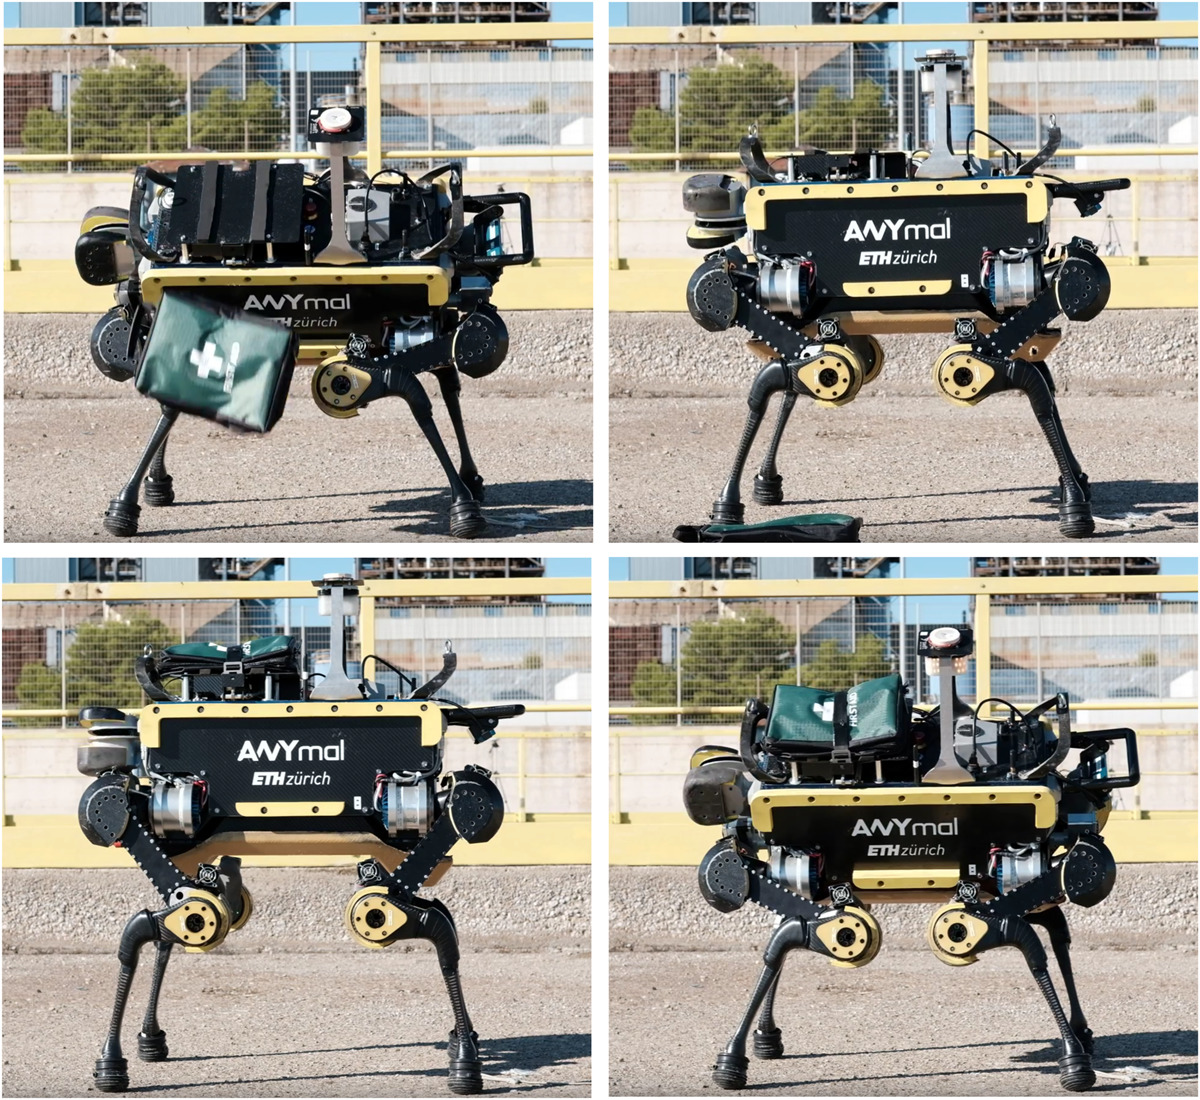
\includegraphics[width=0.8\textwidth]{figures/Payload_delivery.jpg}
    \caption{The ANYmal quadruped robot used in payload delivery applications~\cite{https://doi.org/10.1002/rob.21839}.}
    \label{fig:anymal_payload}
\end{figure}

\section{Legged robot motion control}
\subsection{Biped locomotion design}
\subsection{Inverse/Forward kinematics}
Inverse and Forward Kinematics are mathematical formulas used to calculate the position and configuration of a robot actuator. Forward kinematics is the process of calculating the position and orientation of the end effector based on known joint parameters(angles or displacements). Inverse kinematics is the process of determining the joint parameters needed to achieve a desired position and orientation of the end effector. 

\textbf{Denavit-Hartenberg convention} is a commonly used method for obtaining the forward kinematics model of serial manipulators and simplifying the kinematic analysis. The convention is based on using 4 parameters for each joint to define the relative transformation between coordinate frames attached to adjacent links of a robot manipulator:
\begin{itemize}
  \item \textbf{\( \theta_i \)} -- Joint angle: rotation around the \( z_{i-1} \) axis.
  \item \textbf{\( d_i \)} -- Link offset: translation along the \( z_{i-1} \) axis.
  \item \textbf{\( a_i \)} -- Link length: translation along the \( x_i \) axis (distance between \( z_{i-1} \) and \( z_i \)).
  \item \textbf{\( \alpha_i \)} -- Link twist: rotation around the \( x_i \) axis (angle between \( z_{i-1} \) and \( z_i \)).
\end{itemize}

Each of these parameters defines a physical feature of the robot joint. Three of these parameters will always remain static and the fourth parameter will be dynamic depending on the type of joint. The joints can be simple or more complex. In this case, we focus on hinge joints that rotate around a single axis and prismatic joints that permit linear motion along a single axis. In this thesis, we simply focus on joints with one degree-of-freedom.
To perform the kinematic analysis, we rigidly attach a coordinate frame to each link. In order to represent any arbitrary homogeneous transformation using only four parameters, we must apply 2 constraints:

\begin{itemize}
  \item The axis $x_{i-1}$ is perpendicular to the axis $z_i$
  \item The axis $x_i$ intersects the axis $z_{i-1}$
\end{itemize}

After setting up a system of axes following the constraints, we can calculate the forward kinematics for all joints. With this conversion, each transformation $A_i$ is represented as a product of four basic transformations.

% Requires: \usepackage{amsmath}
\begin{equation}
\begin{aligned}
    A_i &= R_{z,\theta_i} \, \text{Trans}_{z,d_i} \, \text{Trans}_{x,a_i} \, R_{x,\alpha_i} \\
    &= \begin{bmatrix}
        \cos \theta_i & -\sin \theta_i & 0 & 0 \\
        \sin \theta_i & \cos \theta_i & 0 & 0 \\
        0 & 0 & 1 & 0 \\
        0 & 0 & 0 & 1 \\
    \end{bmatrix}
    \begin{bmatrix}
        1 & 0 & 0 & 0 \\
        0 & 1 & 0 & 0 \\
        0 & 0 & 1 & d_i \\
        0 & 0 & 0 & 1 \\
    \end{bmatrix}
    \begin{bmatrix}
        1 & 0 & 0 & a_i \\
        0 & 1 & 0 & 0 \\
        0 & 0 & 1 & 0 \\
        0 & 0 & 0 & 1 \\
    \end{bmatrix}
    \begin{bmatrix}
        1 & 0 & 0 & 0 \\
        0 & \cos \alpha_i & -\sin \alpha_i & 0 \\
        0 & \sin \alpha_i & \cos \alpha_i & 0 \\
        0 & 0 & 0 & 1 \\
    \end{bmatrix}
    \\
    &= \begin{bmatrix}
        \cos \theta_i & -\sin \theta_i\cos \alpha_i & \sin \theta_i\sin \alpha_i & a_i\cos \theta_i \\
        \sin \theta_i & \cos \theta_i\cos \alpha_i & -\cos \theta_i\sin \alpha_i & a_i\sin \theta_i \\
        0 & \sin \alpha_i & \cos \alpha_i & d_i \\
        0 & 0 & 0 & 1 \\
    \end{bmatrix}
\end{aligned}
\end{equation}
From here we can form the overall transformation matrix as a product of the homogeneous transformation matrices:
\begin{equation}
   T_n^0 = A_1 A_2 \cdots A_n
\label{placeholder}
\end{equation}


\section{Expressive Robot motion control}
The relationship between robot movement and our perception has been an exciting and recognized area of research \cite{van_den_brule_robot_2014}. Robots are highly capable and are used in a wide variety of situations. When placed in environments where they interact with humans, they have an innate ability to communicate with their human counterparts. Even when disregarding verbal communication, robots are able to communicate through movement and use their embodiment to generate expressive movements in addition to completing tasks. Using expressive and communicative movements, robots can provide additional information to their human partners.

The general approach to motion control is done through developing trajectories and controllers that produce fast, accurate, and smooth motion while maintaining high repeatability in controlled environments. This is typically done through feedback control loops that allow the robot to react to its environment.  This approach to control is most commonly applied in industrial settings where robot manipulators operate with a fixed or mobile base operating in isolation from humans. The resulting motion will be rather machine-like, as it moves with consistent motion in straight lines. We have also seen that motion control for legged robotic systems has been an active area of research\cite{wieber_modeling_2016}. When working with legged systems, the focus of developing trajectories and control becomes more challenging as we also have to maintain balance, which is especially challenging in biped robots.

Robots are now being used outside isolated industrial settings and are increasingly expected to interact with humans in contexts like interactive art, companionship, collaboration, and assistance. These new applications introduce new challenges in motion generation as the performance can no longer be evaluated by objective criteria like precision and speed, but rather by the perception of the user.

\subsection{Animating robots}
When developing algorithms for expressive motions, there are multiple areas of research from which to draw inspiration. The field of character animation has mastered the art of endowing digital characters with the illusion of life. Bringing this level of lifelike expression to robots has been an aspiration for some time. An approach proposed by Van Breemen in \cite{breemen_bringing_2004} suggests applying the principles of character animation to bring robots to life. Breemen also presented an animation engine that combines multiple interactive robot behaviors with believable robot animations\cite{van_breemen_animation_2004}. Takayama et al. built further on this idea in \cite{takayama_expressing_2011} and found that drawing from animation principles allowed the robot to illustrate forethought and reaction. This was also found to make people more sure of their interpretations of the robot's behavior while also making the robot appear more appealing, approachable, capable, and intelligent even when failing functional tasks at hand. 

In the work of Thomas and Johnson \cite{thomas_disney_1981}, they documented how Walt Disney Studios practices their methods of animation until they derived a series of methods that produced predictable results. These methods were then deemed the fundamental principles of animation. These principles are not verified by science but are widely used in a variety of animated media. The principles are as follows: 
\begin{itemize}
    \item \textbf{Squash and Stretch:} Characters and objects should squash and stretch with their action, although they do not completely lose their shape. 
    \item \textbf{Anticipation:} Major action should be telegraphed such as reaching back before throwing an object. 
    \item \textbf{Staging:} An action should be clear to the audience. For example, the audience should understand the action by only viewing it in silhouette.
    \item \textbf{Straight Ahead Action and Pose to Pose:} This principle describes how to draw an action. Drawing straight ahead involves starting to draw and simple continuing until the action is completed. Pose to pose implies that specific poses are desired in an action and are choreographed before the actual animation.
    \item \textbf{Slow In and Slow Out:} The speed of a motion is not the same during the time that it is performed. Action is slower at the beginning and end. 
    \item \textbf{Arcs:} Move limbs in arcs as opposed to of straight up-down and left-right motions. 
    \item \textbf{Secondary Action:} Create complementary actions that emphasize the main action. For example, a character puts on a coat while walking out the door. 
    \item \textbf{Timing:} Changes in number of frames that are between a start and stop determines the speed of the action, thereby increasing the number of frames and decreasing the speed of the action. 
    \item \textbf{Exaggeration:} Exaggerated action ensures that it is easier to understand the feelings of a character. 
    \item \textbf{Solid Drawing:} Drawings should look plausible and three-dimensional and twinssymmetrical limbs on a character—should be avoided, since it makes characters look stiff.
    \item \textbf{Appeal:} All the characters should be appealing whether one is expected to sympathize with them or despise them. 
\end{itemize}

These principles can also be employed by physical systems in order to make systems appear more lifelike. While the field offers a wide range of techniques, this section focuses on a subset that is particularly relevant to the goals of this project.

Commonly applied principles include \textit{Secondary action} and are applied in \cite{park_generation_2015} to help provide increased readability and credibility of behaviors and expressions of robots. Similar principles are applied in the work of Asselborn et al. \cite{asselborn_keep_2017} they explored the effects of a robot's subconscious gestures made during moments when idle on the perception of children. In the conclusion of this work, a clear correlation was found between the adaptor movements and the humanity and friendliness perception. 

Other principles being used in robot motion include \textit{pose to pose} where a series of key poses are defined first, and the movement between them is generated at a later stage. In Beck et al. \cite{beck_emotional_2012} emotional expressions were constructed by extracting key poses from actor performances, which were then implemented on the Nao robot. Each pose was associated with a specific emotional state validated through user studies. By blending key poses, the robot was enabled to convincingly display emotions through expressive body language.

Other animation principles used to enhance the expressive capabilities of robots include \textit{Exaggeration} and is used to make it easier to interpret what the robot is doing. Exaggeration is utilized with secondary action in \cite{park_generation_2015} in way to make it easier for participants to understand the emotions displayed by the robot.

 
\subsection{Reinforcement learning}
While animation principles can guide the design of expressive robot behaviors, reinforcement learning offers a data-driven framework to generate expressive motion autonomously. Many take advantage of RL when generating expressive motion for robots rather than relying on pre-programmed movements and animations. In the work of Grandia et al. \cite{grandia_design_2024}, reinforcement learning is used to generate expressive motion by training control policies to imitate animations designed by artists. By using a policy gradient approach, the robot character learns perpetual, periodic, and episodic motions based on high-level control commands while still maintaining balance. The reward function is designed to reward accurate movement and survival, enabling the robot to robustly perform expressive motion.
\chapter{Tools and engineering process}
This chapter provides an overview of the tools and processes used throughout the development of Miwo. While the background chapter lays the theoretical groundwork, this chapter focuses on the practical approaches for designing, building, and evaluating the robot. This includes the physical work, such as 3D printing, electronics, and mechanical assembly, as well as the software frameworks and tools used to develop, test, and validate the system.
Table \ref{tab:tools} shows an overview of the tools and software used:

\begin{table}[h]
    \centering
    \begin{tabular}{|l|l|l|}
        \hline
        \textbf{Tool} & \textbf{Name}& \textbf{Version} \\
        \hline
        & & \\[1em]
        \hline
        & & \\[1em]
        \hline
        & & \\[1em]
        \hline
        & & \\[1em]
        \hline
        & & \\[1em]
        \hline
        & & \\[1em]
        \hline
        & & \\[1em]
        \hline
        & & \\[1em]
        \hline
        & & \\[1em]
        \hline
        & & \\[1em]
        \hline
    \end{tabular}
    \caption{Table showing the tools and software used in the work on the thesis.}
    \label{tab:tools}
\end{table}

\newpage
\section*{ROS2}

\section*{3D design (CAD)}
Autodesk Fusion (formerly known as Fusion 360) is a cloud-based platform that combines computer-aided design (CAD), CAM, CAE, and PCB software development into one single tool. It offers a wide range of tools for 3D modeling, design, simulation, and engineering, making it a versatile tool for professionals, researchers, and students. Autodesk Fusion also supports parametric modeling, meaning that design geometry is created using parameters, constraints, and features. This allows designers to change a model's shape instantly by updating it rather than redrawing, ensuring that changes to one part automatically propagate through the entire assembly. All design work for Miwo was carried out in Autodesk Fusion, including structural components, support structures, and body parts that were subsequently 3D printed.

\section*{3D Printing}
3D printing, or additive manufacturing, is a process that allows the creation of three-dimensional objects from digital files by depositing materials layer by layer. 3D printing has grown rapidly in popularity among researchers, professionals, and hobbyists for its potential to enable fast, affordable prototyping across a variety of industries.
During an engineering process, 3D printing allows users to create complex geometries and parts from a wide variety of materials while remaining cost-effective and rapid. With growing popularity and interest, there is a never-ending array of printers, ranging from cheap to expensive, for more detailed and precise work, making them widely accessible.

\section{Electronics and mechanics}

\subsection*{Onboard computer}
The NVIDIA Jetson Orin Nano developer kit is a compact, powerful single-board computer platform from NVIDIA, designed for applications such as generative AI, vision AI, and robotics. It features a powerful ARM-based CPU with an integrated NVIDIA GPU, enabling it to run complex computations without relying on an external power supply. The development board has a small form factor and low power consumption, making it well-suited for portable and embedded robotic systems where weight and size may be constrained. The affordable price point also provides developers, students, and researchers with a powerful and accessible platform. The Jetson Orin nano serves as a suitable onboard computer for mobile robot applications by providing sufficient computing power to run ROS2 nodes and handle communication between the platform's components via USB serial connections.
\subsection*{Servo motors}
Servo motors are rotary actuators that allow for precise control of angular position, velocity, and acceleration. There is a wide variety of servo motors available, ranging from low-cost to high-end professional actuators. Servo motors are used for many robotic applications, such as precise joint control with position feedback or simpler PWM-based alternatives.
\subsection{Go Robot actuators}
\subsection{Power supply}
\subsection{IMU}

\section{Simulation tools and environments}
\subsection{Rviz}
Rviz is a ROS2-compatible 3D visualization tool that allows developers to inspect and debug robotic systems in real time. It provides a user-friendly graphical interface for displaying relevant data, including coordinate frames, joint states, robot models, and sensor data, making it a powerful tool for visualizing the development and testing of robot systems. Rviz works by subscribing to data published to ROS" topics and then rendering them visually, allowing the developer to observe the state of the robot without needing to interact directly with the physical hardware, providing a more intuitive experience.
\subsection{Gazebo}
Gazebo is a powerful open-source 3D robotics simulator compatible with ROS2. Gazebo differs from other pure visualization tools, like Rviz, by providing a powerful physics engine that simulates robots and their interactions with the environment. By using Gazebo, we simulate physical behavior from the ground up, allowing us to model complex physics such as gravity, contact forces, and inertia. This allows the developer to test control algorithms and motion sequences using simulated physics before deploying them on physical hardware.
\subsection{Isaac Sim}
"Isaac Sim is an open source reference framework developed by NVIDIA, built on Omniverse libraries for robotics simulation, testing, and synthetic data generation in physically based virtual environments." Isaac Sim offers physically accurate simulated environments with GPU-accelerated physics and rendering, making it well-suited for applications like reinforcement learning, where large numbers of simulation steps are computed in a short time. Unlike Gazebo, which runs on the CPU, Isaac Sim leverages the
processing capabilities of modern GPUs to run thousands of simulations 
instances almost simultaneously, dramatically accelerating the training process.




\chapter{Implementation}
This chapter provides an overview of the work done to develop the MiWo platform, covering the physical design and construction of the robot, expressive motion design, and locomotion via reinforcement learning
The main goal of this thesis was to construct a robot with a high level of articulation and the capability to communicate emotion and intent through combined movements. Achieving natural and expressive motion across a platform with 16 degrees of freedom requires careful design of both hardware and software. The final platform assumes a biped form-factor as it offers an inherent familiarity to human observers, which is particularly important when evaluating how well the robot communicates emotion and intent. Legged systems also offer a high potential for adaptability and stability in different environments and terrains.

The implementation can be divided into 2 parallel work-streams: the physical system and the software systems that are used to generate motion. The physical/hardware side includes the mechanical design, 3D-printing, electronics, and actuators. The software side covers the ROS2 control architecture, inverse kinematics solvers, expressive motion framework, and the reinforcement learning pipeline used to generate locomotion. 

This chapter begins with the physical design and construction of the robot, followed by the software architecture that ties the system together. Expressive motion design is then presented, covering the kinematics and strategies used for generating the expressive motion. Finally, the reinforcement learning used to derive the gait will be discussed.

\section{Design and construction of robot platform}
\subsection{Leg architecture and design}
The robot stands on 2 legs, and each one is built up with 5 motors, forming a 5 degree-of-freedom kinematic chain. The leg assembly was designed with the goal of having efficient control of the position and orientation of the robot legs relative to the body. Starting from the ground up, the chain begins at the ankle joint, controlling the forward and backward pitch of the foot. Moving upwards, we have the knee joint, responsible for controlling the forward and backward pitch of the lower leg. The upper leg then connects to the hip assembly. 

\textbf{The hip assembly} consists of 3 consecutive joints: hip pitch, hip roll, and hip yaw. One design choice made to simplify the calculations of the inverse and forward kinematics was to construct the hip as a spherical joint. By arranging the 3 rotational axes of the hip joints to intersect at a common point, we are able to simplify the kinematics by decoupling the position and orientation of the legs.

\textbf{The feet} were designed with modularity in mind to conduct testing more easily on different surfaces. Each foot consists of 2 separate parts: An upper component connected directly to the ankle joint and a removable sole that slides smoothly into the upper section and is secured by a small angled 3D-printed peg. The sole section of the foot has a rounded bottom to allow for lateral movement of the body by enabling the robot to shift its weight across the rounded exterior more easily. This design allowed for the possibility of easily replacing or testing different sole geometries. Examples include modifying the degree of rounding underneath the sole or testing different textures or materials for improved grip/stability without needing to reprint the full foot assembly.

\textbf{The shin and femur} link were designed to be intentionally asymmetric with a more organic curvature rather than straight rods. This was done to make the robots appearance more life-like to supplement the expressive goals of the platform. The idea was that having a more natural, animal-like design would contribute to the appearance of the robot and make it feel more alive to the human observers.

\begin{figure}[H]
    \centering
    \includegraphics[width=0.6\textwidth]{Images/leg_architecture.png}
    \caption{The 5 degree-of-freedom leg kinematic chain of Miwo, 
    from ankle pitch through to hip yaw.}
    \label{fig:leg_architecture}
\end{figure}

\subsection{Body Frame and Torso}
The two leg assemblies are connected by a central base link acting as the pelvis and also serving as the structural foundation of the platform. 
\textbf{The Base link} is directly connected to the left and right hip yaw motors and acts as the reference frame for the computation of the kinematics. As this is the central link of the robot, it was designed with the goal of being strong and rigid to support the forces produced by the robots legs.  The base link was also designed to account for testing the kinematics in a safe manner by having a circular hole to accommodate a carbon fiber rod that serves as support when initially testing the inverse kinematics. In addition to the base frame, a small bracket was designed to house a circular linear bearing to allow for smooth, supported vertical motion. To support the carbon fiber rod, a small stand was also designed to keep it straight and allow it to be clamped to a table for increased stability. This was a more novel approach to testing the kinematics, as it was not the ideal material for building a safe and secure test rig; however, all the materials mentioned above were easily available at the time.

\textbf{The internal frame} follows the base frame and can be split into two parts: a lightweight outer frame and a stringer inner frame. The inner frame was designed to provide a larger structural foundation for mounting the outer frame and the neck pitch motor housed in the torso. The outer frame is mounted to the inner frame structure and acts as the scaffolding for supporting the outer shell and housing the internal electronics and cable management within the robot.

\textbf{The internal components} of the torso are organized in the following way: The battery rests on top of the base link to keep a stable center of gravity and is held in place by a thin clamp secured directly to the base link. The clamp secures the rectangular battery on 3 sides, allowing the battery to slide out of the clamp for easy removal by the user. Above the battery is a small basket attached to the outer frame structure, designed to house the internal electronics including the IMU and the DC/DC voltage converter. The backside of the robots torso offers a larger area of free space designed to house the excess length of wires connecting the different electrical components.

\textbf{The outer shell} of the robot was designed to give the robot its final appearance and was mounted directly to the outer frame of the torso. The outer shell was designed to be modular and is separated into 5 different parts. The front and back plates were separated into an upper and lower part to allow for quick reprinting of damaged parts without having to reprint the entire shell. The final part of the outer shell is the section that is mounted directly above the base frame. This part was designed to be easily removed, giving the user easy access to the battery and internal electronics, allowing for service and battery replacement without having to remove the entire outer shell.

\begin{figure}[H]
    \centering
    \includegraphics[width=0.5\textwidth]{Images/body_architecture.png}
    \caption{The body and torso frames of the robot.}
    \label{fig:head_architecture}
\end{figure}

\subsection{Head and Neck Architecture}
The head and neck assembly provides 6 degrees of freedom designed  to allow for a wide range of expressive motions, including nodding, tilting, turning, and secondary actions with antenna movements. The kinematic chain of the upper body begins with the neck pitch motor that is mounted directly to the inner frame of the robots torso.
 
The neck link is responsible for controlling the heads position and was designed to mount directly to the neck pitch motor and to house the head pitch motor, starting the chain that controls the position and orientation of the robots head. At this point in the kinematic chain, the larger robotic actuators are replaced with smaller Dynamixel(XM430) servomotors due to their smaller form factor and the lower torque requirements of the upper body.

\textbf{The head links} are designed to connect the head pitch, yaw, and roll motors that are responsible for controlling the orientation of the robots head. Unlike the hip assembly, the tree head rotation axes do not form a spherical joint. This was a deliberate decision, as the head would be controlled by commanding each of the joint angles directly, making the solving of a full kinematic chain unnecessary, thereby simplifying both the mechanical design and control software.
Designing these links was one of the more challenging aspects of the head assembly. Official dynamixel side-mounting screws are short, constraining the thickness of the links to approximately 1.5 mm, matching the official brackets in metal. To replicate this with PLA proved to be a challenge, as these were the only links that consistently failed during testing. This issue was solved by adding recessed indents around screw holes for better thread engagement, reinforcing high stress areas with supporting structures, and increasing the wall loop count in the slices prior to printing the parts. 


\begin{figure}[H]
    \centering
    \includegraphics[width=0.5\textwidth]{Images/head_architecture.png}
    \caption{The head and neck kinematic chain of Miwo, from neck 
    pitch through to head roll.}
    \label{fig:head_architecture}
\end{figure}

\textbf{The face link} forms the structural base and was designed to be both rigid and lightweight to reduce backlash and strain on the roll, pitch, and yaw motors controlling the head. The face link is mounted directly to the head roll motor and serves as the housing for a significant amount of electrical components. These include: the NVIDIA Orin serving as the onboard computer, two 1.46 inch LCD displays for the eyes, two 9g servos for antenna actuation, an Arduino nano for servo control, a U2D2 board for communicating with the Dynamixel servos, an Adafruit servo driver board, a voltage regulator, and multiple USB cables allowing for serial communication across all components through the NVIDIA Orin nano. The face link was also designed with the mounting of components in a neat manner. Each component would have a dedicated mounting location with either raised screw bosses extruding from the bed of the face link or recessed grooves that allow components to be seated in place before being fastened. Some components required the design of dedicated mounts, such as the two LCD screens and the two 9g servos. Additionally, a series of spare mounting holes were included in the base of the face link to allow for future components to be added without requiring a redesign of the full face link. To finish the design of the head, a removable top cover was designed to be simple, lightweight, and easily removable to access the internal components of the robot.

It should be noted that the face link was originally designed around a different set of internal components. When the initial components did not work as intended, they were replaced, but the face link design was retained as it still provided a sufficient and compatible mounting for the new components. by designing the face link with spare mounting capabilities, it was able to accommodate a change in hardware without having to redesign the full face link.

\begin{figure}[H]
    \centering
    \includegraphics[width=0.5\textwidth]{Images/head_architecture.png}
    \caption{The face link of the robot designed to house the internal components..}
    \label{fig:face_architecture}
\end{figure}

\subsection{Materials and Fabrication}
All structural components and links of the robot platform were fabricated using PLA filament with a Bambu lab A1 or A1 mini 3D printer. PLA was chosen for being affordable, readily available, and lightweight, making it well suited for a platform where weight and accessibility were key priorities in the design process. By fabricating all parts with 3D printing , the cost of the platform was minimized and different iterations could be tested physically within hours of being modeled, supporting the rapid prototyping approach that was used for this project. The use of widely available materials and commercial 3D printers ensures that the platform could be easily replicated by other researchers or developers, in line with the goal of contributing to the research field by making the platform open-source.

\textbf{The assembly} of the final platform uses 3 categories of fasteners depending on the component being attached. All links that were mounted directly to the GO-M8010-r actuators use M3.5 screws for mounting links to the stator and M4 screws for mounting links to the Rotor. The links that are mounted to the Dynamixel XM430 servos use the official mounting screws supplied with the motors The remainder of the assembly was mounted using standard M3 screws in either 10mm or 18.25mm lengths, depending on the required engagement depth.


\section{Software Architecture}
The software system for the Miwo platform was developed on the ROS2 Humble framework running on a device with Ubuntu 22.04. ROS 2 was used because it enables a modular architecture by having individual nodes that communicate by subscribing and publishing data to named channels (topics) or by calling services and actions. This architecture allows the final system to be taken apart into smaller, independently runnable components, facilitating a more comfortable process of development and testing.

the software system can be divided into 3 different hierarchical levels, as illustrated in Figure ~\ref{fig:software_architecture}. The lowest level is responsible for the low-level control of the system and is titled the hardware interface layer. The hardware interface layer consists of a set of bridge nodes. The bridge nodes are responsible for translating the ROS2 commands to low-level motor commands and reading back the hardware state, allowing us to control the hardware directly. One level above sits the state estimator layer, which is responsible for processing the raw sensor data from the IMU and computing the robot's current orientation and body pose. The uppermost layer is the motion control layer, which is responsible for generating body pose commands based on the provided input. The input may come from joystick commands, expressive motion sequencer nodes, or a reinforcement learning policy. The layer is then responsible for translating these commands into the different joint trajectories for each of the motors using an inverse kinematics solver.

\begin{figure}[H]
    \centering
    \fbox{\parbox{0.6\textwidth}{
        \centering
        \vspace{2cm}
        \textit{Figure placeholder — software architecture diagram}
        \vspace{2cm}
    }}
    \caption{Overview of the Miwo software architecture showing 
    the three main layers: hardware interface, state estimation, 
    and motion control.}
    \label{fig:software_architecture}
\end{figure}

\subsection{Hardware Interface Layer}
The hardware interface layer is, as mentioned, responsible for the direct communication between the ROS2 system and the physical actuators of the robot. This layer consists of 5 bridge nodes, each responsible for bridging the ROS2 system and the control protocol of the different actuators.
\textbf{Unitree Motor Bridges}
The Unitree Motor bridges handle the communication between the ROS2 system and the 11 GO-M8010-6 actuators that control the two legs and the neck. There are a total of 3 separate bridges: the left leg, the right leg, and the neck bridge, each communicating with their respective motors split across 2 separate serial ports—one covering the left leg and the other covering the right leg and the neck.

Separating the motors across different serial ports was motivated by 2 main reasons. First, each serial port has a fixed bandwidth, and having all eleven motors on a single connection created a communication bottleneck where motors had to wait for each other before their commands were sent. This introduced latency and jitter into the control loop, causing undesired motion in the system. Second, running each of the bridges across 2 ports with their own control loop would ensure that communication errors on one port or bridge do not block or affect the operation of the other port or bridge. This made it easier to isolate the source of errors and also increased the overall fault tolerance of the system.
Each of the bridge nodes operates with an internal control loop at 50 Hz, receiving joint trajectory commands from the ROS2 controllers and sending low level position, velocity, and torque commands using the Unitree Actuator SDK. The bridge node interpolates the incoming trajectory way-points by using a first order hold scheme for smooth motion. The interpolation is also paired with a low pass filter with a cutoff frequency of 37.5 Hz applied to the motor, similar to the work of \cite{grandia_design_2024}. Joint limits are also enforced in software to prevent commands that could damage the hardware. The Bridge also deploys a gradual gain ramp-up period on startup to further prevent sudden large torques when the motors are first enabled.
The bridges were designed to be started when the robot is placed in its dedicated calibration stand, which holds the robot in a fixed neutral position with the legs fully extended and the neck pitched back. On startup, each bridge will read the current encoder position of all motors and store it as the zero reference point for that run. The following joint angle commands are then interpreted relative to these zero positions instead of using absolute encoder values. This ensures that the robot starts from a consistent and known configuration for each run. This approach was implemented to account for potential encoder drift accumulation or power cycle inconsistencies between runs, which could cause the robot to move to incorrect positions and potentially damage the hardware. Upon startup, there is also a programmed smooth forward pitch so that all Unitree actuators match the zero-position of the urdf file of the robot. 

\textbf{Dynamixel Head Bridge}
The dynamixel head bridge handles the communication between the 3 XM430 servo motors controlling the head roll, pitch, and yaw. The dynamixel motors build a smaller kinematic chain and communicate over a common TTL bus using the Dynamixel SDK and the Dynamixel communication Protocol. The communication between the onboard computer and the servos is handled by a U2D2 USB communication converter. 
The bridge node operates in a similar manner to the Unitree bridge by providing 2 modes depending on the incoming commands. For continuous real-time control, such as joystick input, the bridge subscribes to the joint trajectory commands published to the head controller topic and then translates those commands into Dynamixel position commands. For smooth motion commands, like moving to a predefined pose, the bridge uses a FollowJointTrajectory action server that accepts a goal trajectory and then interpolates smoothly between start and goal positions over a specified period of time.
The node also applies a deadband threshold to incoming position commands to prevent unnecessary motor activity from small or noisy commands. Additional configurations were also applied to the motors prior to deployment, directly on the servo hardware using the official setup wizard. The motors were configured with a smooth motion profile by setting the profile velocity and profile acceleration to low values to generate smooth, pleasant motion. Motor limits were also enforced directly in the setup of the motors.
The logic of the dynamixel bridge differs from the Unitree bridge at startup, as this bridge reads the current position of all three servos and stores them as the initial tracked positions. The 3 servos have predefined idle position values that correspond to the head having 0 degrees of roll, pitch, and yaw. This approach provides a known and previously calibrated neutral head position to which we can command the robot to return when not actively commanding it. If a servo fails for some reason and prevents torque from being enabled on startup, the bridge will automatically attempt to reboot the affected servo before retrying, further increasing the reliability of the startup sequence.
\textbf{}
The antenna bridge is responsible for controlling the two 9g servos that manage the antenna movement of the robot. Unlike the two other bridges that communicate directly with the onboard computer over a serial connection, the antenna servos are driven by an Adafruit PCA9685 16-channel PWM servo driver board. The PCA9685 is a dedicated PWM controller that generates the PWM signals required to position the servo motors. The PCA9685 communicates with an Arduino Nano over the I2C bus, the Arduino receives the position commands from the onboard Jetson over a USB serial connection. This chain of communication (Jetson - Arduino - PCA9685 - Servo) was chosen because the Jetson does not natively generate hardware PWM signals suitable for the servos used, and the Arduino provides a simple and widely available solution for bridging the communication. The bridge node subscribes to joint trajectory messages published to the antenna controller topic and translates the commands into PWM signals forwarded to the Arduino Nano. The Arduino runs a dedicated script that forwards the PWM signals received to the PCA9685, updating the servo positions. The antennas are not involved in the balance or inverse kinematics of the robot and act independently, allowing for movement to be layered on top of other motions. In the context of expressive motion, the antenna motion will serve as a secondary action previously mentioned in the animation principles.
\textbf{Eye Control Node}
The robots eyes are controlled from the onboard computer with an independent node. The node communicates with the two LCD displays over Wi-Fi, sending expression commands that correspond to a predefined set of different expressions like [happy, sad, squint, angry, idle]. The node also supplies the robot with realistic blinking by periodically publishing a blink command at random intervals with a randomized set of different blink animations, including [fast blink, single eye blink, slow blink, asymmetrical blink], which have different weights, to give a more lifelike blinking experience. In addition to sending out blink signals, the node also subscribes to an eye command topic, allowing the later discussed animation nodes to publish eye commands at specific parts of of longer expressive motions.

\subsection{State Estimation}
\subsubsection{IMU Pipeline}
\subsubsection{Robot State Node}
\subsection{Body Pose Control}
\subsubsection{Cartesian Body Controller}
\subsubsection{Leveling Node}

\section{Expressive Motion Design}
\subsection{Forward Kinematics}
\subsection{Inverse Kinematics}
\subsection{Motion Primitives}
\subsection{Expressive Motion Design}
\subsection{Motion Sequencer}

\section{Locomotion via Reinforcement Learning}
\subsection{Simulation environment setup}
\subsection{Observation and action space}
\subsection{Reward function design}
\subsection{Training setup and hyper-parameters}

\chapter{User experiments}
This chapter presents the experiments conducted to evaluate the 2 contributions of the Miwo platform. The main focus is the evaluation of the expressive motion framework, but it also presents progress in RL locomotion. 

Evaluating the overall expressiveness of a robot is different from evaluating other robotic systems. The performance cannot be evaluated by objective metrics alone. If a motion is technically smooth and precise but fails to communicate the intended emotion or intent, it must be considered unsuccessful. To accurately evaluate the expressive capabilities of Miwo, we rely on a Human perception study in which participants are asked to classify and evaluate different expressive motions either by interacting directly with the physical robot or by watching short video clips of the robot performing each motion. 

In addition to the human perception trials, this chapter will also cover the experiments and results related to the RL locomotion. 


\section{Experiment design and Participants}
The experiment was designed to evaluate the MiWo robot's overall expressive capabilities through a human perception study. Participants initially encountered the robot in an idle state before being presented with 6 different expressive motions. After each animation, the participants were asked to classify what emotion or intent they believed the robot was expressing. Participants were also asked to evaluate the overall impression of the robot after all 6 motions were completed. This study employed a questionnaire-based design to collect responses, and quantitative methods were used to assess the clarity of expressive motions.

\subsection{Experiment setup}               
The participants of the study can be divided into two groups based on how they experienced the robot's expressive motions: 
The first group attended live demonstrations, where they observed the physical robot performing directly in front of them, allowing them to get a better impression of its size, mechanics, and weight. 
The second group completed the experiments remotely by watching short video clips of the same motions performed in the live demonstrations. 
By offering both in-person and remote participant options, the study was accessible to a broader range of participants. The responses of the 2 groups were also analyzed separately to identify any differences in the perception between live and video-based observations.
                
\subsection{Participants}
Participants were recruited using a wide variety of methods. The participants for the live demonstrations were mostly recruited by asking fellow students and researchers available on campus. Recruitment for the video-based study involved creating multiple social media posts, posting posters around campus, and sending direct invitations to the study to various friends and family, resulting in a wide range of participants with diverse backgrounds.
A total of 38 participants completed the study: 16 attended the live demonstration, and 22 completed the remote video-based study. The participants were not required to have any prior knowledge of robotics or engineering, and no demographic restrictions were imposed other than a minimum age requirement. Before participating in the study, all participants were informed of its purpose and provided consent. All responses were collected anonymously using a participant ID system that could not be linked back to individual participants, and no personal data was collected. Data was stored securely and used solely for academic research purposes in accordance with the institution's data management policy.

\begin{figure}[H]
\centering

\begin{subfigure}[t]{0.48\textwidth}
\centering
{\small\textbf{Live study (N=16)}}
\vspace{1.0cm}

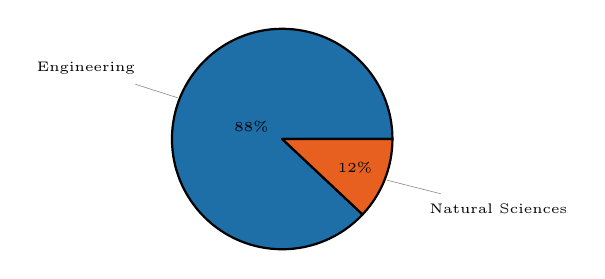
\begin{tikzpicture}[scale=0.7]
\pie[
    color={navyblue, emotion},
    text=pin,
    before number=,
    after number=\%,
    font=\tiny,
    radius=2,
]
{88/Engineering, 12/Natural Sciences}
\end{tikzpicture}

\vspace{1.0cm}
{\small \textbf{Field of study}}
\vspace{0.8cm}

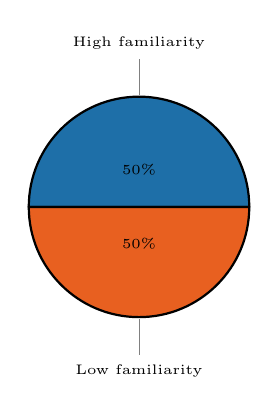
\begin{tikzpicture}[scale=0.7]
\pie[
    color={navyblue, emotion},
    text=pin,
    before number=,
    after number=\%,
    font=\tiny,
    radius=2,
]
{50/High familiarity, 50/Low familiarity}
\end{tikzpicture}

\vspace{0.5cm}
{\small \textbf{Robot familiarity}}
\end{subfigure}
\hfill
\begin{subfigure}[t]{0.48\textwidth}
\centering
{\small\textbf{Video study (N=22)}}
\vspace{0.1cm}

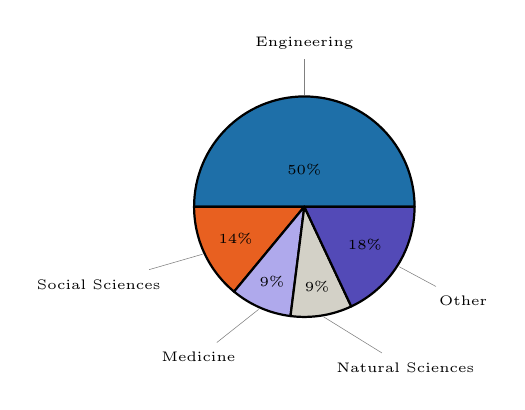
\begin{tikzpicture}[scale=0.7]
\pie[
    color={navyblue, emotion, adjacent, lightgrey, intended},
    text=pin,
    before number=,
    after number=\%,
    font=\tiny,
    radius=2,
]
{50/Engineering, 14/Social Sciences,
 9/Medicine, 9/Natural Sciences, 18/Other}
\end{tikzpicture}

\vspace{0.1cm}
{\small \textbf{Field of study}}
\vspace{0.8cm}

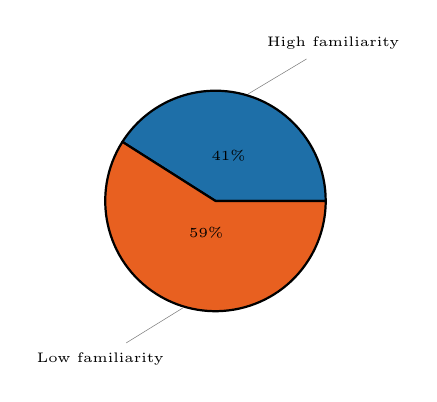
\begin{tikzpicture}[scale=0.7]
\pie[
    color={navyblue, emotion},
    text=pin,
    before number=,
    after number=\%,
    font=\tiny,
    radius=2,
]
{41/High familiarity, 59/Low familiarity}
\end{tikzpicture}

\vspace{0.6cm}
{\small \textbf{Robot familiarity}}
\end{subfigure}

\caption[Demographic breakdown of participants]{Demographic breakdown of participants. The top row shows
Field of study distribution, the bottom row shows robot familiarity
grouped into high (moderately familiar, very familiar, or expert)
and low (not familiar or slightly familiar).}
\label{fig:demographics_pie}
\end{figure}

% bar/pie chart for participants and demographics
As shown in \autoref{fig:demographics_pie}, the two groups differ noticeably in their respective backgrounds. The live study group, consisting of participants found on campus, is almost exclusively from engineering and technology fields, making up 88\% of participants. This displays potential weakness in the campus-based recruitment process. The video-based study shows a more diverse distribution, with only 50\% of participants doing engineering. Other differences include the live-study group reporting a higher level of overall robot familiarity, with 50\% rating themselves as having a higher level of familiarity compared to the 41\% in the video-based studies. These demographic differences are acknowledged as potential factors in interpreting the performance differences between the two studies and are addressed further in the results chapter.


\subsection{Procedure and questionnaire} 
In the first part, where participants experienced the robot live, they entered the room to find it already turned on and in an idle state, performing breathing-like, subtle movements. To provide a similar experience to the group in the video-based study, participants were first asked to watch a one-minute video of the robot standing and moving in its idle state, allowing them to familiarize themselves with the robot's idle behavior and appearance, ensuring that the following animations were evaluated relative to the robot's idle state rather than isolated movements without context. Each participant was then presented with 6 video clips or live demonstrations of the robot performing distinct expressive motions. The motions presented were designed to correspond to the following emotions or intents: Curiosity, Happiness, Sadness, Disappointment, Anger, and Fear. For each motion, participants were asked to answer 4 questions. The first question asked participants to name the emotion or intent the robot was expressing in their own words, with no predefined options, allowing for more open-ended responses. This was followed by 3 questions asking the participants to rate their confidence in their answers, how well they felt the robot expressed the named emotion, and how natural the motion felt on a scale of 1 to 5.

\begin{table}[H]
\centering
\begin{tabular}{|l|l|l|}
    \hline
    \textbf{Question} & \textbf{Type} & \textbf{Scale} \\
    \hline
    Q1. What emotion or intent does the robot & Open-ended & Free text \\
    appear to be expressing? & & \\
    \hline
    Q2. How confident are you in your answer? & Likert scale & 1 -- 5 \\
    \hline
    Q3. How well do you think the robot & Likert scale & 1 -- 5 \\
    expressed this emotion? & & \\
    \hline
    Q4. How natural did the robot's & Likert scale & 1 -- 5 \\
    movement feel? & & \\
    \hline
\end{tabular}
\caption{Questions the participants were faced with during the emotion/intent recognition part of the study.}
\label{tab:questionnaire}
\end{table}

The open-ended format for the question regarding emotion/intent recognition was deliberately chosen to avoid influencing participants into a predefined set of options. By doing so, we allow for a more genuine assessment of whether the intended emotion/intent was communicated clearly without guiding the participant to a specific answer.

Following the individual evaluation, participants would provide an overall evaluation of the robot using the Godspeed scale. The Godspeed scale was introduced in \cite{bartneck_measurement_2008} as a standardized instrument for measuring human-robot interactions and is widely used and recognized. The Godspeed scale evaluates perceptions of the robot across 5 key concepts in HRI: anthropomorphism, animacy, likability, perceived intelligence, and perceived safety. Each concept is assessed using 5 consistent questionnaires that employ semantic differential scales. Using a standardized, validated metric for the overall evaluation allows the study's results to be compared with other work in expressive robotics and human-robot interaction.

The order of the motions was the same for each participant, and the questionnaire was administered digitally using Google Forms for both the live and video-based studies, taking approximately 10-15 minutes to complete.

\subsection{Metrics and evaluation}
It is worth noting that the study collects two categories of data. The emotion/intent recognition data consist of open-ended labels, which were analyzed by grouping responses into emotion/intent categories and calculating recognition rates for each animation. The scaled responses for analyzing confidence, expressiveness, and naturalness were analyzed quantitatively, while the godspeed scale data were scored and analyzed per dimension.

Due to the open-ended nature of the emotion/intent recognition question, responses were grouped into three categories for better visualization and quantitative analysis. The response groups include: intended emotion (response matching the intended emotion), adjacent emotion (response describing a related or overlapping emotional state), and other (responses unrelated to the intended emotion). Grouping participants' responses was necessary to enable quantitative comparisons across animations while preserving the insights of the open-ended response format. 
An example of the grouping logic can be seen in the curiosity animation. One participant classified the animation as \textbf{'cautious-}, this was classified as adjacent since caution shares the attentive qualities of the curiosity animation, even if it does not directly match the name of the intended emotion. 




\chapter{Results}
This chapter presents the results from the human perception study. The results are organized into 3 sections, each covering emotion/intent recognition, Likert-scale ratings, and Godspeed questionnaire results. Where relevant, the results of the live study (N=16) and video-based study (N=22) are presented separately and compared to identify any differences in perception between the two approaches.

\section{Emotion Recognition Results}
This section presents the results of the open-ended emotion recognition task, in which participants were asked to describe the emotion or intent the robot was conveying in each of the 6 expressive animations. As previously mentioned, the responses were divided into 3 groups: \textit{intended}, \textit{adjacent}, or \textit{other}. Figure~\ref{fig:recognition_rate} summarizes the recognition rate, i.e., the rate at which the responses were categorized as the intended emotion. IT shows the recognition rates across all six animations for both the live and video-based groups, followed by a detailed breakdown of the response distribution in figures~\ref{fig:emotion_recognition_live} and ~\ref{fig:emotion_recognition_video}.

%\newpage
\begin{figure}[H]
\centering
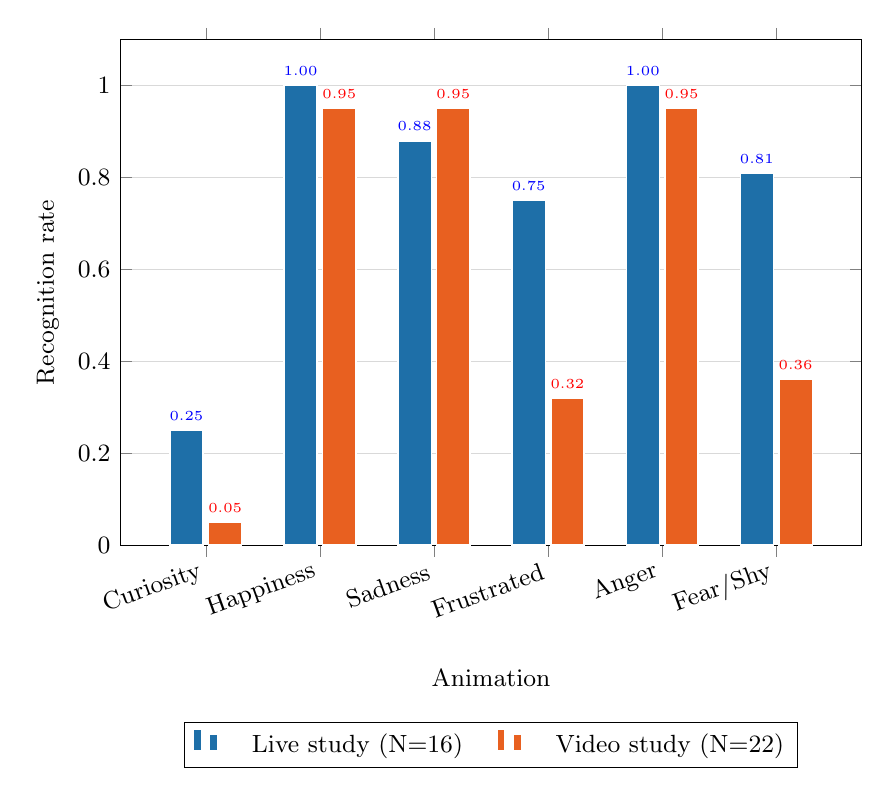
\begin{tikzpicture}
\begin{axis}[
    ybar,
    bar width=12pt,
    width=11cm,
    height=8cm,
    ymin=0, ymax=1.1,
    ytick={0, 0.2, 0.4, 0.6, 0.8, 1.0},
    ylabel={Recognition rate},
    xlabel={Animation},
    xtick=data,
    symbolic x coords={A1, A2, A3, A4, A5, A6},
    xticklabels={
        {Curiosity},
        {Happiness},
        {Sadness},
        {Frustrated},
        {Anger},
        {Fear/Shy}
    },
    x tick label style={
        font=\small,
        rotate=20,
        anchor=east,
        yshift=-4pt,
    },
    legend style={
        at={(0.5,-0.35)},
        anchor=north,
        legend columns=2,
        font=\small,
        column sep=10pt,
    },
    enlarge x limits=0.15,
    tick label style={font=\small},
    label style={font=\small},
    xlabel style={yshift=-10pt},
    ymajorgrids=true,
    grid style={line width=0.2pt, draw=gray!30},
    nodes near coords,
    nodes near coords align={vertical},
    every node near coord/.append style={font=\tiny},
    point meta=explicit symbolic,
]

% Live study — navy
\addplot+[ybar, fill=navyblue, draw=white, line width=0.5pt]
    coordinates {
        (A1, 0.25) [0.25]
        (A2, 1.00) [1.00]
        (A3, 0.88) [0.88]
        (A4, 0.75) [0.75]
        (A5, 1.00) [1.00]
        (A6, 0.81) [0.81]
    };

% Video study — orange
\addplot+[ybar, fill=emotion, draw=white, line width=0.5pt]
    coordinates {
        (A1, 0.05) [0.05]
        (A2, 0.95) [0.95]
        (A3, 0.95) [0.95]
        (A4, 0.32) [0.32]
        (A5, 0.95) [0.95]
        (A6, 0.36) [0.36]
    };

\legend{Live study (N=16), Video study (N=22)}

\end{axis}
\end{tikzpicture}
\caption[Emotion recognition rates per animation for the live
study]{Emotion recognition rates per animation for the live
study (N=11) and video-based study (N=22). Values represent
The percentage of participants who correctly identified the
intended emotion.}
\label{fig:recognition_rate}
\end{figure}

By examining these results, a clear distinction between the animations can be seen. Some animations were more consistently recognized, while others proved more ambiguous in interpretation. \textit{Happiness} and \textit{Anger} achieve near-perfect scores in both live and video-based studies, with live rates of 100\% and video rates of 95\%. Sadness also offers a high recognition rate, with 88\% in the live study and 95\% in the video-based study. The \textit{Curiosity} animation was the weakest performer overall, achieving recognition rates of 25\% in the live study and only 5\% in the video-based study. Results also show that the live study consistently outperformed the video-based study across all animations, except for the \textit{sadness} animation. A notable performance gap was also observed for \textit{Disappointment} (75\% live vs.\ 32\% video) and \textit{Fear} 
(81\% live vs.\ 36\% video), which are examined in detail below.

Figure ~\ref{fig:emotion_recognition_video} shows how the different responses were classified for each of the 6 emotions. \textit{Anger}, \textit{Happiness}, and \textit{Frustrated} show a low level of variation consistent with their high recognition rates. The remaining 3 animations display a wider variety of answers, indicating that participants interpreted them differently.




\begin{figure}[H]
\centering
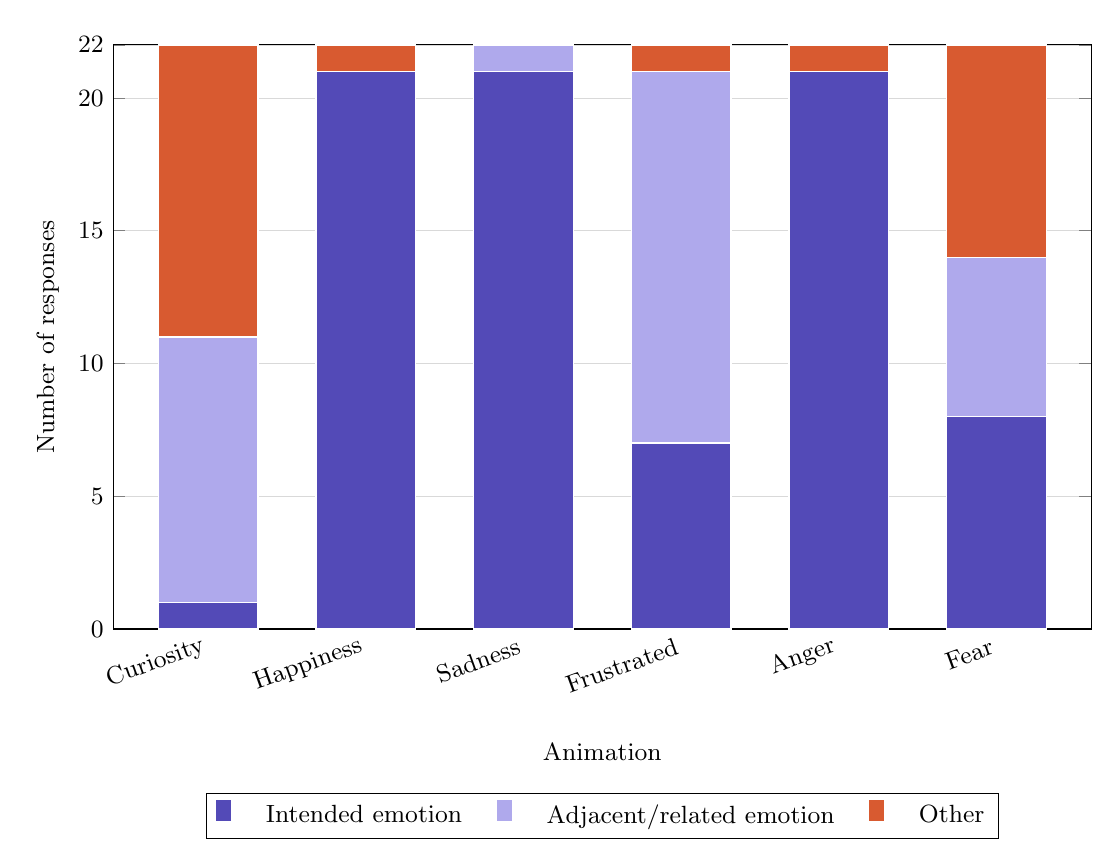
\begin{tikzpicture}
\begin{axis}[
    ybar stacked,
    bar width=36pt,
    width=14cm,
    height=9cm,
    ymin=0, ymax=22,
    ytick={0,5,10,15,20,22},
    ylabel={Number of responses},
    xlabel={Animation},
    xtick=data,
    symbolic x coords={A1, A2, A3, A4, A5, A6},
    xticklabels={
        {Curiosity},
        {Happiness},
        {Sadness},
        {Frustrated},
        {Anger},
        {Fear}
    },
    x tick label style={
        font=\small,
        rotate=20,
        anchor=east,
        yshift=-5pt,
    },
    legend style={
        at={(0.5,-0.28)},
        anchor=north,
        legend columns=3,
        font=\small,
        column sep=10pt,
    },
    enlarge x limits=0.12,
    tick label style={font=\small},
    label style={font=\small},
    xlabel style={yshift=-10pt},
    ymajorgrids=true,
    grid style={line width=0.2pt, draw=gray!30},
]

\addplot+[ybar, fill=intended, draw=white, line width=0.5pt]
    coordinates {
        (A1, 1)(A2, 21)(A3, 21)(A4, 7)(A5, 21)(A6, 8)
    };

\addplot+[ybar, fill=adjacent, draw=white, line width=0.5pt]
    coordinates {
        (A1, 10)(A2, 0)(A3, 1)(A4, 14)(A5, 0)(A6, 6)
    };

\addplot+[ybar, fill=other, draw=white, line width=0.5pt]
    coordinates {
        (A1, 11)(A2, 1)(A3, 0)(A4, 1)(A5, 1)(A6, 8)
    };

\legend{
    Intended emotion,
    Adjacent/related emotion,
    Other
}

\end{axis}
\end{tikzpicture}
\caption[Emotion recognition results in video-based study]{Distribution of emotion recognition responses across all six
animations for the video-based study (N=22). Responses were grouped
into three categories: intended emotion (matching the target),
adjacent/related emotion (overlapping emotional state), and other
(unrelated responses). Dark purple indicates correct identification
of the intended emotion.}
\label{fig:emotion_recognition_video}
\end{figure}
\newpage
\begin{figure}[H]
\centering
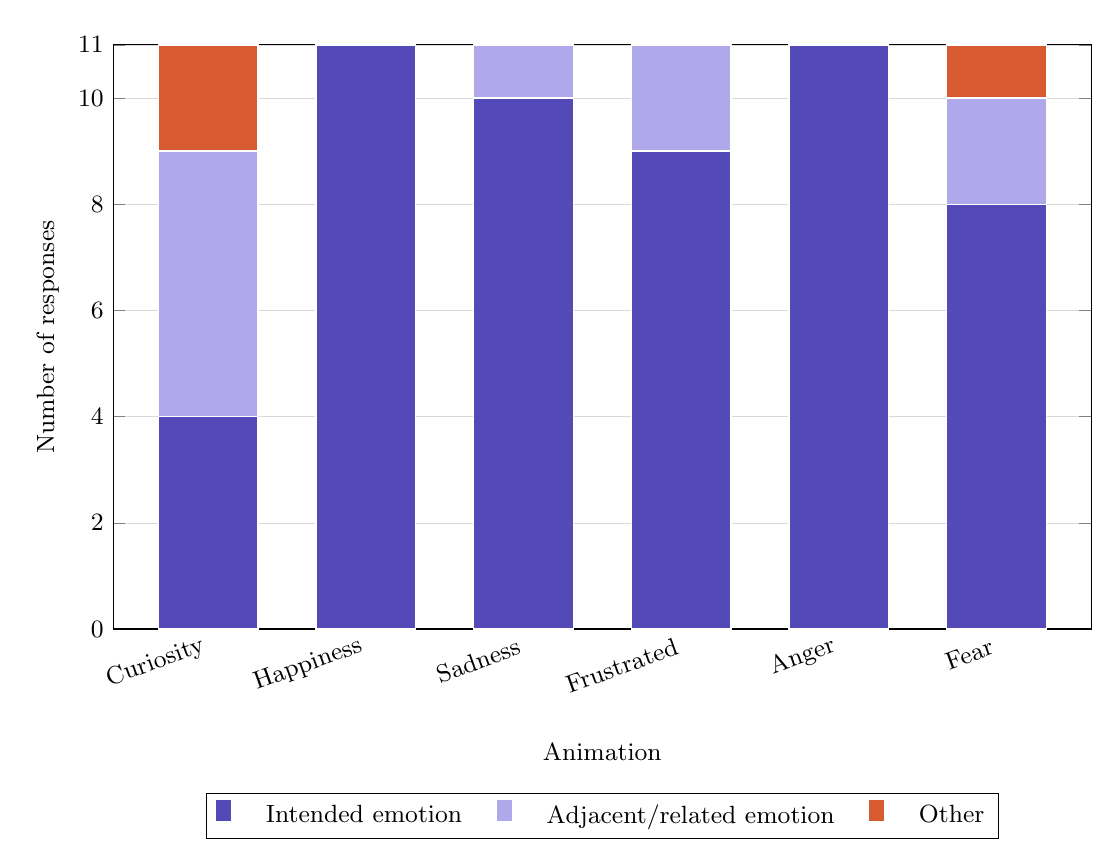
\begin{tikzpicture}
\begin{axis}[
    ybar stacked,
    bar width=36pt,
    width=14cm,
    height=9cm,
    ymin=0, ymax=11,
    ytick={0,2,4,6,8,10,11},
    ylabel={Number of responses},
    xlabel={Animation},
    xtick=data,
    symbolic x coords={A1, A2, A3, A4, A5, A6},
    xticklabels={
        {Curiosity},
        {Happiness},
        {Sadness},
        {Frustrated},
        {Anger},
        {Fear}
    },
    x tick label style={
        font=\small,
        rotate=20,
        anchor=east,
        yshift=-5pt,
    },
    legend style={
        at={(0.5,-0.28)},
        anchor=north,
        legend columns=3,
        font=\small,
        column sep=10pt,
    },
    enlarge x limits=0.12,
    tick label style={font=\small},
    label style={font=\small},
    xlabel style={yshift=-10pt},
    ymajorgrids=true,
    grid style={line width=0.2pt, draw=gray!30},
]

\addplot+[ybar, fill=intended, draw=white, line width=0.5pt]
    coordinates {
        (A1, 4)(A2, 11)(A3, 10)(A4, 9)(A5, 11)(A6, 8)
    };

\addplot+[ybar, fill=adjacent, draw=white, line width=0.5pt]
    coordinates {
        (A1, 5)(A2, 0)(A3, 1)(A4, 2)(A5, 0)(A6, 2)
    };

\addplot+[ybar, fill=other, draw=white, line width=0.5pt]
    coordinates {
        (A1, 2)(A2, 0)(A3, 0)(A4, 0)(A5, 0)(A6, 1)
    };

\legend{
    Intended emotion,
    Adjacent/related emotion,
    Other
}

\end{axis}
\end{tikzpicture}
\caption{Distribution of emotion recognition responses across all six
animations for the live study (N=11). Responses were grouped
into three categories: intended emotion (matching the target),
adjacent/related emotion (overlapping emotional state), and other
(unrelated responses). Dark purple indicates correct identification
of the intended emotion.}
\label{fig:emotion_recognition_live}
\end{figure}
\textbf{Curiosity} had the highest concentration of responses categorized as \textit{other}, with recurring answers including confusion, tiredness, sadness, and frustration. This was also the weakest performing animation overall, achieving recognition rates of only 25\% in the live study and 5\% in the video-based study.

\textbf{Frustrated} had the highest concentration of \textit{adjacent} responses while still having a very low concentration of \textit{other} responses. Recurring answers included impatience, disgust, and feeling upset.

\textbf{Fear} also displayed a wide spread of responses across all three categories. In the live study, 81\% of participants correctly identified the intended emotion, whereas the video-based study achieved only 36\%, representing the largest gap between the two groups, particularly for \textit{Frustrated}. Recurring adjacent responses included shyness, sadness, and surprise.





\newpage
\section{Likert Scale Results}
% Confidence, expressiveness, naturalness per animation

\begin{figure}[H]
\centering
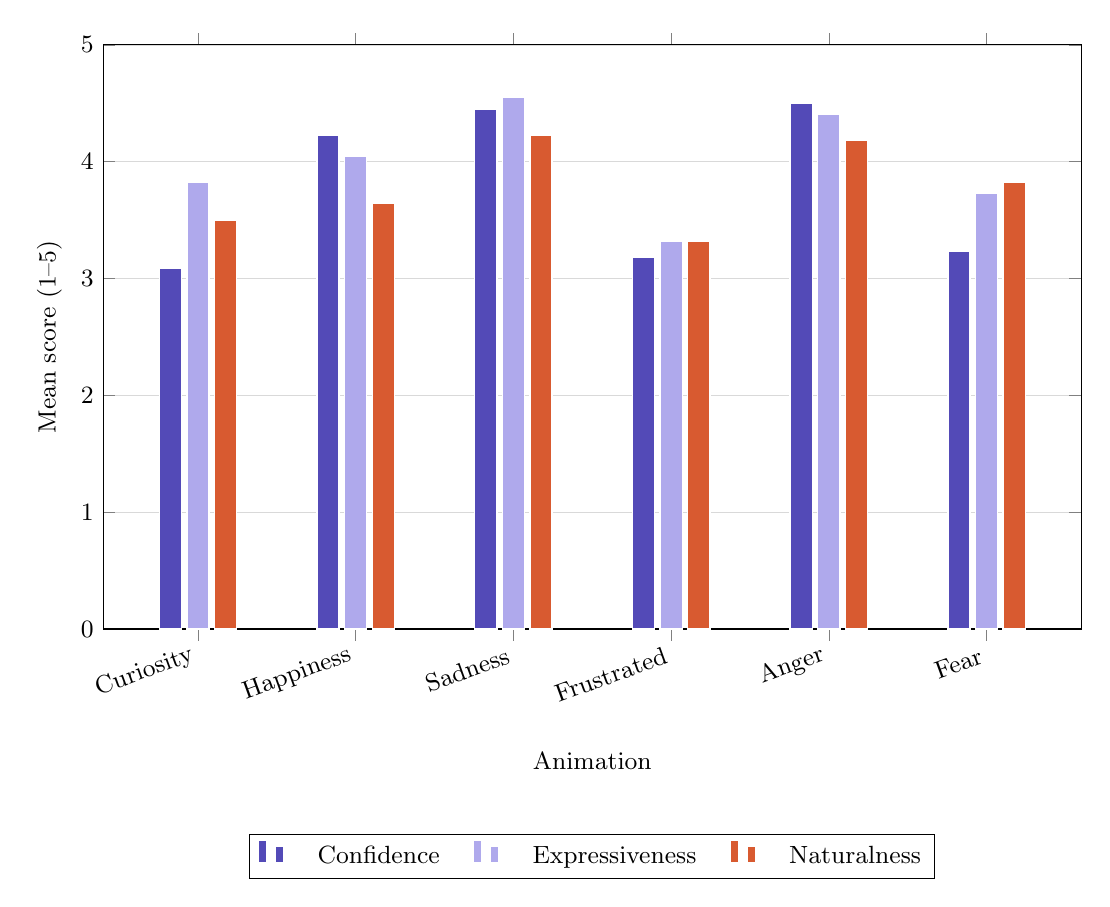
\begin{tikzpicture}
\begin{axis}[
    ybar,
    bar width=8pt,
    width=14cm,
    height=9cm,
    ymin=0, ymax=5,
    ytick={0,1,2,3,4,5},
    ylabel={Mean score (1--5)},
    xlabel={Animation},
    xtick=data,
    symbolic x coords={A1, A2, A3, A4, A5, A6},
    xticklabels={
        {Curiosity},
        {Happiness},
        {Sadness},
        {Frustrated},
        {Anger},
        {Fear}
    },
    x tick label style={
        font=\small,
        rotate=20,
        anchor=east,
        yshift=-4pt,
    },
    legend style={
        at={(0.5,-0.35)},
        anchor=north,
        legend columns=3,
        font=\small,
        column sep=10pt,
    },
    enlarge x limits=0.12,
    tick label style={font=\small},
    label style={font=\small},
    xlabel style={yshift=-10pt},
    ymajorgrids=true,
    grid style={line width=0.2pt, draw=gray!30},
]

% Confidence — dark purple
\addplot+[ybar, fill=intended, draw=white, line width=0.5pt]
    coordinates {
        (A1,3.09)(A2,4.23)(A3,4.45)(A4,3.18)(A5,4.50)(A6,3.23)
    };

% Expressiveness — lavender
\addplot+[ybar, fill=adjacent, draw=white, line width=0.5pt]
    coordinates {
        (A1,3.82)(A2,4.05)(A3,4.55)(A4,3.32)(A5,4.41)(A6,3.73)
    };

% Naturalness — orange
\addplot+[ybar, fill=other, draw=white, line width=0.5pt]
    coordinates {
        (A1,3.50)(A2,3.64)(A3,4.23)(A4,3.32)(A5,4.18)(A6,3.82)
    };

\legend{
    Confidence,
    Expressiveness,
    Naturalness
}

\end{axis}
\end{tikzpicture}
\caption{Mean Likert scale scores per animation for the video-based 
study (N=22). Each animation shows three bars representing mean 
confidence, expressiveness, and naturalness ratings on a scale of 
1 to 5.}
\label{fig:likert_video}
\end{figure}
\begin{figure}[H]
\centering
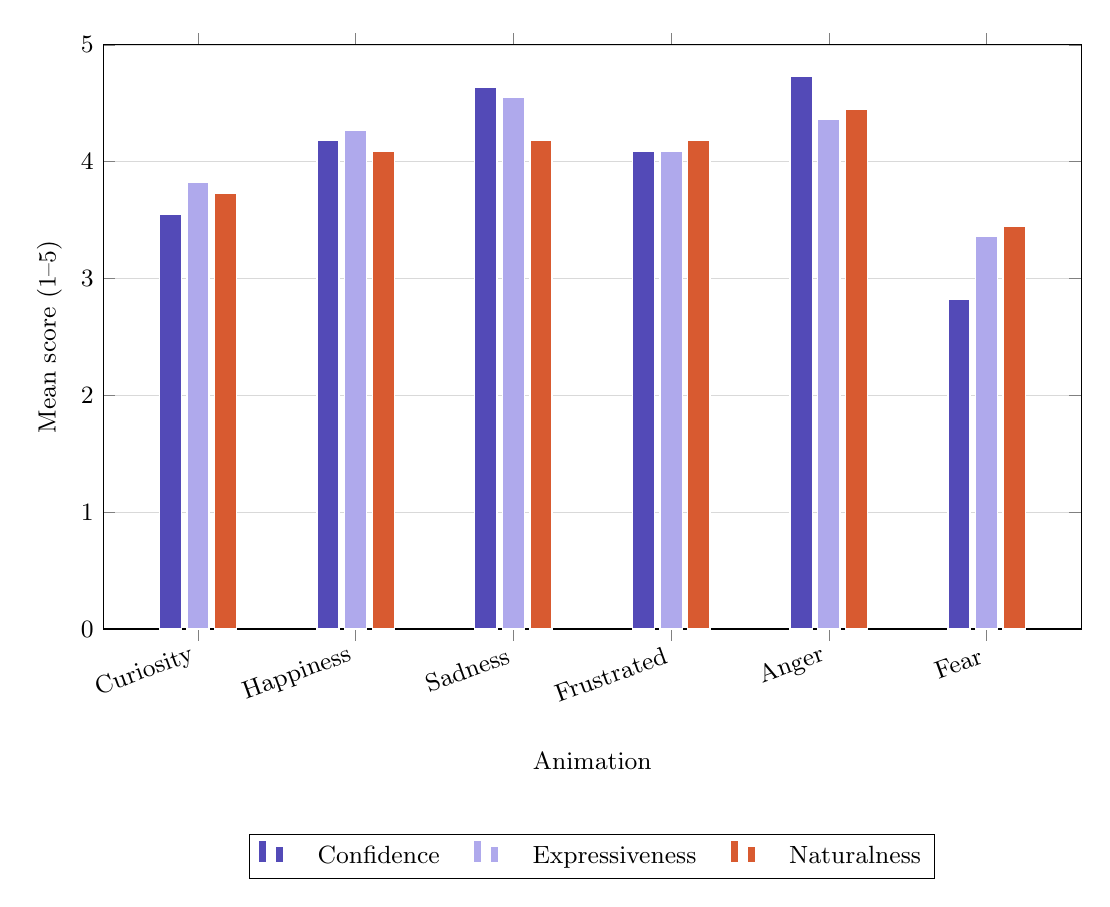
\begin{tikzpicture}
\begin{axis}[
    ybar,
    bar width=8pt,
    width=14cm,
    height=9cm,
    ymin=0, ymax=5,
    ytick={0,1,2,3,4,5},
    ylabel={Mean score (1--5)},
    xlabel={Animation},
    xtick=data,
    symbolic x coords={A1, A2, A3, A4, A5, A6},
    xticklabels={
        {Curiosity},
        {Happiness},
        {Sadness},
        {Frustrated},
        {Anger},
        {Fear}
    },
    x tick label style={
        font=\small,
        rotate=20,
        anchor=east,
        yshift=-4pt,
    },
    legend style={
        at={(0.5,-0.35)},
        anchor=north,
        legend columns=3,
        font=\small,
        column sep=10pt,
    },
    enlarge x limits=0.12,
    tick label style={font=\small},
    label style={font=\small},
    xlabel style={yshift=-10pt},
    ymajorgrids=true,
    grid style={line width=0.2pt, draw=gray!30},
]

% Confidence — dark purple
\addplot+[ybar, fill=intended, draw=white, line width=0.5pt]
    coordinates {
        (A1,3.55)(A2,4.18)(A3,4.64)(A4,4.09)(A5,4.73)(A6,2.82)
    };

% Expressiveness — lavender
\addplot+[ybar, fill=adjacent, draw=white, line width=0.5pt]
    coordinates {
        (A1,3.82)(A2,4.27)(A3,4.55)(A4,4.09)(A5,4.36)(A6,3.36)
    };

% Naturalness — orange
\addplot+[ybar, fill=other, draw=white, line width=0.5pt]
    coordinates {
        (A1,3.73)(A2,4.09)(A3,4.18)(A4,4.18)(A5,4.45)(A6,3.45)
    };

\legend{
    Confidence,
    Expressiveness,
    Naturalness
}

\end{axis}
\end{tikzpicture}
\caption[Mean Likert scale scores per animation for the live 
study]{Mean Likert scale scores per animation for the live 
study (N=11). Each animation shows three bars representing mean 
confidence, expressiveness, and naturalness ratings on a scale of 
1 to 5.}
\label{fig:likert_live}
\end{figure}




\subsection*{Godspeed Results}
% Five dimensions ( spider chart)
\begin{figure}[H]
\centering
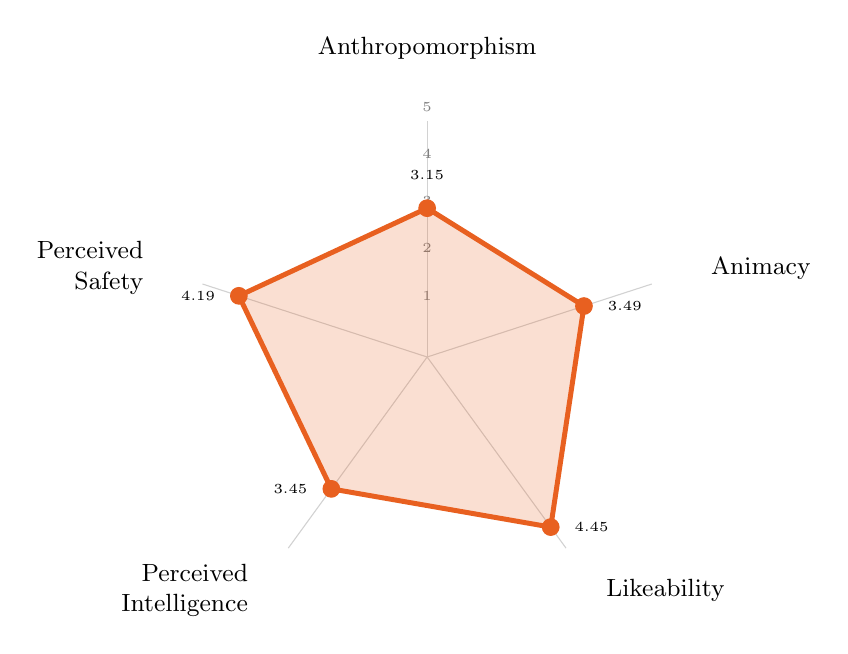
\begin{tikzpicture}[scale=3.0]
\def\N{5}
\def\levels{5}
% Colors
\colorlet{spiderline}{emotion}
\colorlet{spiderfill}{emotion}
% Axis labels and values
\def\labels{{"Anthropomorphism", "Animacy", "Likeability", 
             "Perceived\\Intelligence", "Perceived\\Safety"}}
\def\values{{3.15, 3.49, 4.45, 3.45, 4.19}}
% Draw background grid rings
\foreach \lev in {1,...,5}{
    \draw[gray!25, line width=0.4pt]
        \foreach \i in {1,...,5}{
            -- ({(\lev/5)*cos(90+(\i-1)*360/5)},
               {(\lev/5)*sin(90+(\i-1)*360/5)})
        } -- cycle;
}
% Draw axis lines
\foreach \i in {1,...,5}{
    \draw[gray!35, line width=0.4pt]
        (0,0) -- ({cos(90+(\i-1)*360/5)}, {sin(90+(\i-1)*360/5)});
}
% Draw tick labels on one axis (right side)
\foreach \lev in {1,...,5}{
    \node[font=\tiny, gray] at 
        ({(\lev/5)*cos(90)}, {(\lev/5)*sin(90)+0.06}) {\lev};
}
% Plot data — video study
\fill[spiderfill, opacity=0.2]
    ({(3.15/5)*cos(90)},   {(3.15/5)*sin(90)})   --
    ({(3.49/5)*cos(90-72)}, {(3.49/5)*sin(90-72)}) --
    ({(4.45/5)*cos(90-144)},{(4.45/5)*sin(90-144)}) --
    ({(3.45/5)*cos(90-216)},{(3.45/5)*sin(90-216)}) --
    ({(4.19/5)*cos(90-288)},{(4.19/5)*sin(90-288)}) --
    cycle;
\draw[spiderline, line width=1.8pt]
    ({(3.15/5)*cos(90)},   {(3.15/5)*sin(90)})   --
    ({(3.49/5)*cos(90-72)}, {(3.49/5)*sin(90-72)}) --
    ({(4.45/5)*cos(90-144)},{(4.45/5)*sin(90-144)}) --
    ({(3.45/5)*cos(90-216)},{(3.45/5)*sin(90-216)}) --
    ({(4.19/5)*cos(90-288)},{(4.19/5)*sin(90-288)}) --
    cycle;
% Data point dots
\foreach \val/\angle in {
    3.15/90, 3.49/18, 4.45/-54, 3.45/-126, 4.19/-198}{
    \filldraw[spiderline] 
        ({(\val/5)*cos(\angle)}, {(\val/5)*sin(\angle)}) 
        circle (1pt);
}
% Value labels next to dots
\node[font=\tiny, above] at 
    ({(3.15/5)*cos(90)+0.0},   {(3.15/5)*sin(90)+0.08})   {3.15};
\node[font=\tiny, right] at 
    ({(3.49/5)*cos(18)+0.06},  {(3.49/5)*sin(18)})        {3.49};
\node[font=\tiny, right] at 
    ({(4.45/5)*cos(-54)+0.06}, {(4.45/5)*sin(-54)})       {4.45};
\node[font=\tiny, left] at 
    ({(3.45/5)*cos(-126)-0.06},{(3.45/5)*sin(-126)})      {3.45};
\node[font=\tiny, left] at 
    ({(4.19/5)*cos(-198)-0.06},{(4.19/5)*sin(-198)})      {4.19};
% Axis labels
\node[font=\small, above, align=center] at 
    ({1.22*cos(90)},   {1.22*sin(90)})    {Anthropomorphism};
\node[font=\small, right, align=left] at 
    ({1.22*cos(18)},   {1.22*sin(18)})    {Animacy};
\node[font=\small, right, align=left] at 
    ({1.22*cos(-54)},  {1.22*sin(-54)})   {Likeability};
\node[font=\small, left, align=right] at 
    ({1.22*cos(-126)}, {1.22*sin(-126)})  {Perceived\\Intelligence};
\node[font=\small, left, align=right] at 
    ({1.22*cos(-198)}, {1.22*sin(-198)})  {Perceived\\Safety};
\end{tikzpicture}
\caption{Godspeed questionnaire results for the video-based study 
(N=22) across five dimensions. Scores are on a scale of 1 to 5.}
\label{fig:godspeed_video}
\end{figure} 

\begin{figure}[H]
\centering
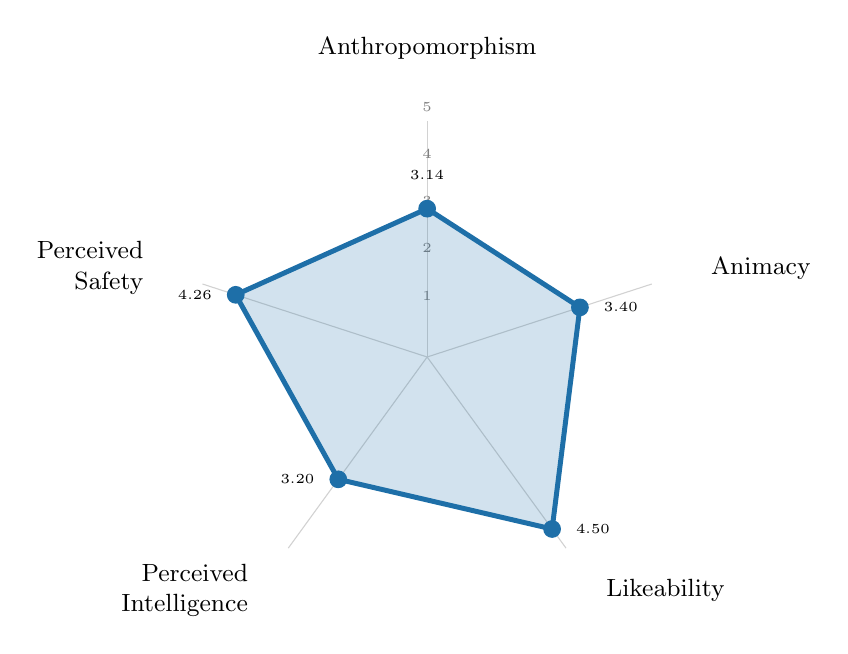
\begin{tikzpicture}[scale=3.0]
\def\N{5}
\def\levels{5}
% Colors
\colorlet{spiderline}{navyblue}
\colorlet{spiderfill}{navyblue}
% Draw background grid rings
\foreach \lev in {1,...,5}{
    \draw[gray!25, line width=0.4pt]
        \foreach \i in {1,...,5}{
            -- ({(\lev/5)*cos(90+(\i-1)*360/5)},
               {(\lev/5)*sin(90+(\i-1)*360/5)})
        } -- cycle;
}
% Draw axis lines
\foreach \i in {1,...,5}{
    \draw[gray!35, line width=0.4pt]
        (0,0) -- ({cos(90+(\i-1)*360/5)}, {sin(90+(\i-1)*360/5)});
}
% Draw tick labels
\foreach \lev in {1,...,5}{
    \node[font=\tiny, gray] at 
        ({(\lev/5)*cos(90)}, {(\lev/5)*sin(90)+0.06}) {\lev};
}
% Plot data — live study N=16
\fill[spiderfill, opacity=0.2]
    ({(3.14/5)*cos(90)},   {(3.14/5)*sin(90)})   --
    ({(3.40/5)*cos(90-72)}, {(3.40/5)*sin(90-72)}) --
    ({(4.50/5)*cos(90-144)},{(4.50/5)*sin(90-144)}) --
    ({(3.20/5)*cos(90-216)},{(3.20/5)*sin(90-216)}) --
    ({(4.26/5)*cos(90-288)},{(4.26/5)*sin(90-288)}) --
    cycle;
\draw[spiderline, line width=1.8pt]
    ({(3.14/5)*cos(90)},   {(3.14/5)*sin(90)})   --
    ({(3.40/5)*cos(90-72)}, {(3.40/5)*sin(90-72)}) --
    ({(4.50/5)*cos(90-144)},{(4.50/5)*sin(90-144)}) --
    ({(3.20/5)*cos(90-216)},{(3.20/5)*sin(90-216)}) --
    ({(4.26/5)*cos(90-288)},{(4.26/5)*sin(90-288)}) --
    cycle;
% Data point dots
\foreach \val/\angle in {
    3.14/90, 3.40/18, 4.50/-54, 3.20/-126, 4.26/-198}{
    \filldraw[spiderline] 
        ({(\val/5)*cos(\angle)}, {(\val/5)*sin(\angle)}) 
        circle (1pt);
}
% Value labels
\node[font=\tiny, above] at 
    ({(3.14/5)*cos(90)+0.0},   {(3.14/5)*sin(90)+0.08})   {3.14};
\node[font=\tiny, right] at 
    ({(3.40/5)*cos(18)+0.06},  {(3.40/5)*sin(18)})        {3.40};
\node[font=\tiny, right] at 
    ({(4.50/5)*cos(-54)+0.06}, {(4.50/5)*sin(-54)})       {4.50};
\node[font=\tiny, left] at 
    ({(3.20/5)*cos(-126)-0.06},{(3.20/5)*sin(-126)})      {3.20};
\node[font=\tiny, left] at 
    ({(4.26/5)*cos(-198)-0.06},{(4.26/5)*sin(-198)})      {4.26};
% Axis labels
\node[font=\small, above, align=center] at 
    ({1.22*cos(90)},   {1.22*sin(90)})    {Anthropomorphism};
\node[font=\small, right, align=left] at 
    ({1.22*cos(18)},   {1.22*sin(18)})    {Animacy};
\node[font=\small, right, align=left] at 
    ({1.22*cos(-54)},  {1.22*sin(-54)})   {Likeability};
\node[font=\small, left, align=right] at 
    ({1.22*cos(-126)}, {1.22*sin(-126)})  {Perceived\\Intelligence};
\node[font=\small, left, align=right] at 
    ({1.22*cos(-198)}, {1.22*sin(-198)})  {Perceived\\Safety};
\end{tikzpicture}
\caption[Godspeed questionnaire results for the live-based study]{Godspeed 
questionnaire results for the live study (N=16) across five dimensions. 
Scores are on a scale of 1 to 5.}
\label{fig:godspeed_live}
\end{figure}

\begin{figure}[H]
\centering
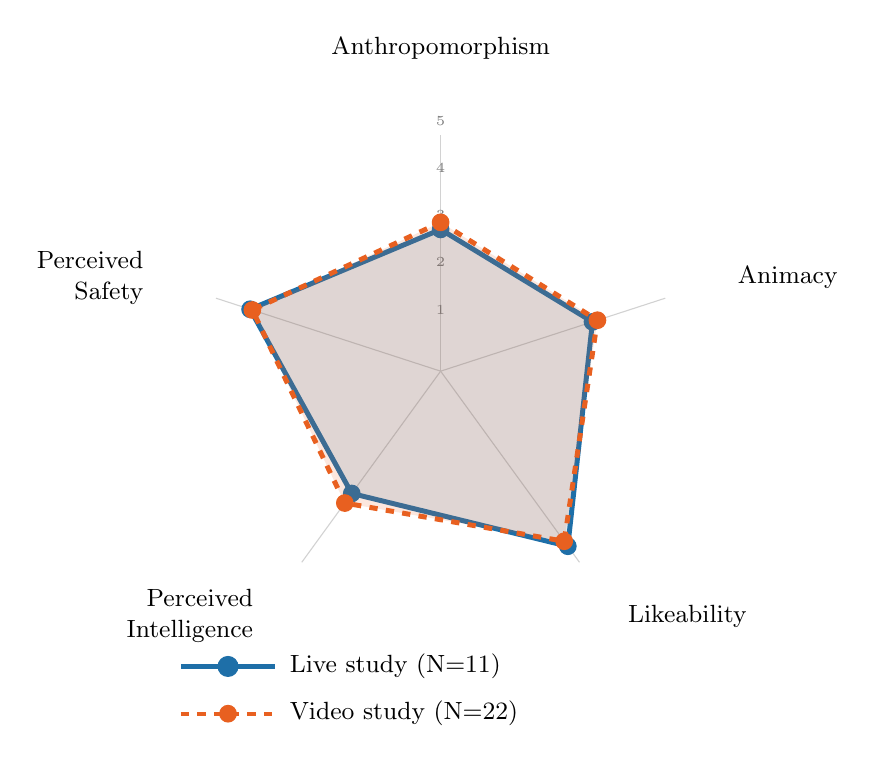
\begin{tikzpicture}[scale=3.0]

\foreach \lev in {1,...,5}{
    \draw[gray!25, line width=0.4pt]
        \foreach \i in {1,...,5}{
            -- ({(\lev/5)*cos(90+(\i-1)*360/5)},
               {(\lev/5)*sin(90+(\i-1)*360/5)})
        } -- cycle;
}
\foreach \i in {1,...,5}{
    \draw[gray!35, line width=0.4pt]
        (0,0) -- ({cos(90+(\i-1)*360/5)}, {sin(90+(\i-1)*360/5)});
}
\foreach \lev in {1,...,5}{
    \node[font=\tiny, gray] at
        ({(\lev/5)*cos(90)}, {(\lev/5)*sin(90)+0.06}) {\lev};
}

% Live — navy solid
\fill[navyblue, opacity=0.15]
    ({(3.00/5)*cos(90)},   {(3.00/5)*sin(90)})   --
    ({(3.38/5)*cos(18)},   {(3.38/5)*sin(18)})   --
    ({(4.58/5)*cos(-54)},  {(4.58/5)*sin(-54)})  --
    ({(3.20/5)*cos(-126)}, {(3.20/5)*sin(-126)}) --
    ({(4.24/5)*cos(-198)}, {(4.24/5)*sin(-198)}) --
    cycle;
\draw[navyblue, line width=1.8pt]
    ({(3.00/5)*cos(90)},   {(3.00/5)*sin(90)})   --
    ({(3.38/5)*cos(18)},   {(3.38/5)*sin(18)})   --
    ({(4.58/5)*cos(-54)},  {(4.58/5)*sin(-54)})  --
    ({(3.20/5)*cos(-126)}, {(3.20/5)*sin(-126)}) --
    ({(4.24/5)*cos(-198)}, {(4.24/5)*sin(-198)}) --
    cycle;
\foreach \val/\angle in {
    3.00/90, 3.38/18, 4.58/-54, 3.20/-126, 4.24/-198}{
    \filldraw[navyblue]
        ({(\val/5)*cos(\angle)}, {(\val/5)*sin(\angle)}) circle (1.0pt);
}

% Video — orange dashed
\fill[emotion, opacity=0.15]
    ({(3.15/5)*cos(90)},   {(3.15/5)*sin(90)})   --
    ({(3.49/5)*cos(18)},   {(3.49/5)*sin(18)})   --
    ({(4.45/5)*cos(-54)},  {(4.45/5)*sin(-54)})  --
    ({(3.45/5)*cos(-126)}, {(3.45/5)*sin(-126)}) --
    ({(4.19/5)*cos(-198)}, {(4.19/5)*sin(-198)}) --
    cycle;
\draw[emotion, line width=1.8pt, dashed]
    ({(3.15/5)*cos(90)},   {(3.15/5)*sin(90)})   --
    ({(3.49/5)*cos(18)},   {(3.49/5)*sin(18)})   --
    ({(4.45/5)*cos(-54)},  {(4.45/5)*sin(-54)})  --
    ({(3.45/5)*cos(-126)}, {(3.45/5)*sin(-126)}) --
    ({(4.19/5)*cos(-198)}, {(4.19/5)*sin(-198)}) --
    cycle;
\foreach \val/\angle in {
    3.15/90, 3.49/18, 4.45/-54, 3.45/-126, 4.19/-198}{
    \filldraw[emotion]
        ({(\val/5)*cos(\angle)}, {(\val/5)*sin(\angle)}) circle (1.0pt);
}

% Axis labels
\node[font=\small, above, align=center] at ({1.28*cos(90)},{1.28*sin(90)})   {Anthropomorphism};
\node[font=\small, right, align=left]   at ({1.28*cos(18)},{1.28*sin(18)})   {Animacy};
\node[font=\small, right, align=left]   at ({1.28*cos(-54)},{1.28*sin(-54)}) {Likeability};
\node[font=\small, left, align=right]   at ({1.28*cos(-126)},{1.28*sin(-126)}) {Perceived\\Intelligence};
\node[font=\small, left, align=right]   at ({1.28*cos(-198)},{1.28*sin(-198)}) {Perceived\\Safety};

% Legend
\draw[navyblue, line width=1.5pt] (-1.1,-1.25) -- (-0.7,-1.25);
\filldraw[navyblue] (-0.9,-1.25) circle (1.2pt);
\node[font=\small, right] at (-0.68,-1.25) {Live study (N=11)};

\draw[emotion, line width=1.5pt, dashed] (-1.1,-1.45) -- (-0.7,-1.45);
\filldraw[emotion] (-0.9,-1.45) circle (1.0pt);
\node[font=\small, right] at (-0.68,-1.45) {Video study (N=22)};

\end{tikzpicture}
\caption{Godspeed questionnaire results for both study groups across
five dimensions. Solid line represents the live study (N=11) and
dashed line represents the video-based study (N=22).
Scores are on a scale of 1 to 5.}
\label{fig:godspeed_overlay}
\end{figure}





%\section{RL Locomotion Experiments}
%\subsection{Simulation experiments}
%\subsubsection{Gait performance in simulation}
%\subsubsection{Hardware gait performance}
\chapter{Discussion}

\section{General discussion}

\section{Conclusion}

\section{Future works}


\chapter{Conclusion}
The work completed in this thesis was motivated by the following three research objectives: 
\begin{enumerate}
    \item Design and construct a highly articulated bipedal robot platform capable of producing a wide range of expressive motions using accessible and commonly available manufacturing methods and hardware components.

    \item Develop a software framework for generating and executing expressive motion on the platform, capable of producing a diverse range of motions that clearly communicate distinct emotions and intents.

    \item Evaluate the expressive capabilities of the platform through a human perception study, assessing the degree to which independent observers can reliably identify the intended emotion from the robot's motion alone.
\end{enumerate}

To achieve the above research objectives. In contrast, this thesis presents the design, construction, and evaluation of MiWo, an open-source bipedal robot platform for expressive human-robot interaction. The platform was constructed entirely from 3D-printed PLA components and commercially available actuators, sensors, and other components. The resulting platform is a 16-DOF system capable of coordinated full-body motion. As a further contribution to the research field, the CAD files, code, and documentation were all released as open source, allowing the platform to be replicated or built upon by other researchers or developers. 

A ROS2 software framework was developed for controlling the robot and for designing and executing expressive motion. The final framework combines an analytical inverse kinematics solver with handcrafted animation nodes, each responsible for conveying an emotional state or intent. The animation nodes were designed with principles drawn from character animation, including anticipation, slow-in and slow-out, secondary action, and exaggeration. The resulting framework produced coordinated motion sequences across the full kinematic chain, with complementary eye expressions and antenna movements used as secondary actions to further enhance the expressive capabilities of the robot. The robot was equipped with six different animations, each designed to communicate a distinct emotion or intent clearly.

The expressive capabilities of the platform were evaluated through human perception studies involving 38 participants across a live (N=16) and a video-based (N=22) study groups. The Animations corresponding to basic emotions, including \textit{Happiness}, \textit{Fear}, \textit{Sadness}, and \textit{Anger}, achieved high-scoring recognition rates in one or both study groups. In contrast, more cognitively complex states such as \textit{Curiosity} and \textit{Frustrated} proved more ambiguous, yielding lower scores in recognition rates.  Likert scale results confirmed that naturalness received consistent scores across all animations, suggesting that motion quality was not a limiting factor for the weaker animations, but rather their motion design. Likert scale results also produced consistently high scores in both confidence and naturalness for the basic emotions, showing that the robot was capable of expressing a range of emotions with confidence. The Godspeed questionnaire 
revealed a high likability and perceived safety, with a high degree of consistency between the two groups, further demonstrating the robot's potential for human-robot interactions.

The results of the studies demonstrate that a small, open-source, 3D-printed biped robot is capable of communicating a range of emotional states through motion in a manner that is reliably recognized and positively perceived by human observers. It can be argued that the robot can, with a high recognition rate, communicate basic emotions, but emotional or cognitive states that are more ambiguous were not recognized at the same level. The work carried out in this thesis contributes to the research field by providing a fully documented, accessible platform with a set of evaluated expressive animations, offering a sturdy foundation for further research and development into motion design and human-robot interactions.
\input{chapters/09_Future_Work}

% Back matter
\backmatter{}
\printbibliography{}

% Appendices
\appendix


\end{document}